\documentclass[10pt]{beamer}\usepackage[]{graphicx}\usepackage[]{color}
% maxwidth is the original width if it is less than linewidth
% otherwise use linewidth (to make sure the graphics do not exceed the margin)
\makeatletter
\def\maxwidth{ %
  \ifdim\Gin@nat@width>\linewidth
    \linewidth
  \else
    \Gin@nat@width
  \fi
}
\makeatother

\definecolor{fgcolor}{rgb}{0.345, 0.345, 0.345}
\newcommand{\hlnum}[1]{\textcolor[rgb]{0.686,0.059,0.569}{#1}}%
\newcommand{\hlstr}[1]{\textcolor[rgb]{0.192,0.494,0.8}{#1}}%
\newcommand{\hlcom}[1]{\textcolor[rgb]{0.678,0.584,0.686}{\textit{#1}}}%
\newcommand{\hlopt}[1]{\textcolor[rgb]{0,0,0}{#1}}%
\newcommand{\hlstd}[1]{\textcolor[rgb]{0.345,0.345,0.345}{#1}}%
\newcommand{\hlkwa}[1]{\textcolor[rgb]{0.161,0.373,0.58}{\textbf{#1}}}%
\newcommand{\hlkwb}[1]{\textcolor[rgb]{0.69,0.353,0.396}{#1}}%
\newcommand{\hlkwc}[1]{\textcolor[rgb]{0.333,0.667,0.333}{#1}}%
\newcommand{\hlkwd}[1]{\textcolor[rgb]{0.737,0.353,0.396}{\textbf{#1}}}%
\let\hlipl\hlkwb

\usepackage{framed}
\makeatletter
\newenvironment{kframe}{%
 \def\at@end@of@kframe{}%
 \ifinner\ifhmode%
  \def\at@end@of@kframe{\end{minipage}}%
  \begin{minipage}{\columnwidth}%
 \fi\fi%
 \def\FrameCommand##1{\hskip\@totalleftmargin \hskip-\fboxsep
 \colorbox{shadecolor}{##1}\hskip-\fboxsep
     % There is no \\@totalrightmargin, so:
     \hskip-\linewidth \hskip-\@totalleftmargin \hskip\columnwidth}%
 \MakeFramed {\advance\hsize-\width
   \@totalleftmargin\z@ \linewidth\hsize
   \@setminipage}}%
 {\par\unskip\endMakeFramed%
 \at@end@of@kframe}
\makeatother

\definecolor{shadecolor}{rgb}{.97, .97, .97}
\definecolor{messagecolor}{rgb}{0, 0, 0}
\definecolor{warningcolor}{rgb}{1, 0, 1}
\definecolor{errorcolor}{rgb}{1, 0, 0}
\newenvironment{knitrout}{}{} % an empty environment to be redefined in TeX

\usepackage{alltt}


%\input{slides_header.tex}
\usepackage{graphicx}
\usepackage{hyperref, url}
\hypersetup{colorlinks,citecolor=myorange,filecolor=red,linkcolor=brown,urlcolor=blue}

\usepackage{longtable,booktabs}
\usepackage{amssymb,amsmath}
\usepackage{animate}
\usepackage{subfig}
\usepackage{tikz}
\usetikzlibrary{shapes.geometric, arrows,shapes.symbols,decorations.pathreplacing}
\tikzstyle{startstop} = [rectangle, rounded corners, minimum width=3cm, minimum height=1cm, draw=black, fill=pinkish,text width=3.5cm]
\tikzstyle{startstop2} = [rectangle, rounded corners, minimum width=3cm, minimum height=1cm, draw=black, fill=background,text width=4.5cm]
\tikzstyle{startstop3} = [rectangle, rounded corners, minimum width=3cm, minimum height=1cm, draw=black, fill=beige,text width=3.0cm]
\tikzstyle{startstop4} = [rectangle, rounded corners, minimum width=3cm, minimum height=1cm, draw=black, fill=pinkish,text width=4.5cm]
\tikzstyle{io} = [trapezium, trapezium left angle=70, trapezium right angle=110, minimum width=2cm, minimum height=1cm, text centered, draw=black, fill=blue!30,text width=1.5cm]
\tikzstyle{process} = [rectangle, minimum width=1cm, minimum height=1cm, text centered, draw=black, fill=orange!30,text width=2cm]
\tikzstyle{decision} = [diamond, minimum width=2cm, minimum height=1cm, text centered, draw=black, fill=green!30]
\tikzstyle{arrow} = [thick,->,>=stealth]
\tikzstyle{both} = [thick,<->,>=stealth, red]


% used for tree of stats tests in 001-introduction
\tikzstyle{startstopstats} = [rectangle, rounded corners, minimum width=2cm, minimum height=.5cm,text centered, draw=black, fill=red!30]
\tikzstyle{iostats} = [trapezium, trapezium left angle=70, trapezium right angle=110, minimum width=2cm, minimum height=.5cm, text centered, draw=black, fill=blue!30]
\tikzstyle{processstats} = [rectangle, minimum width=1.5cm, minimum height=.5cm, text centered, draw=black, fill=orange!30]
\tikzstyle{processbigstats} = [rectangle, minimum width=1.5cm, minimum height=.5cm, text centered, draw=black, fill=orange!30,text width=1.6cm]
\tikzstyle{decisionstats} = [rectangle, minimum width=1cm, minimum height=1cm, text centered, draw=black, fill=green!30,text width=1.6cm]
\tikzstyle{decisionbigstats} = [rectangle, minimum width=1cm, minimum height=1cm, text centered, draw=black, fill=yellow!30,text width=2cm]

\usepackage{pifont}% http://ctan.org/pkg/pifont
\newcommand{\cmark}{\ding{51}}%
\newcommand{\xmark}{\ding{55}}%

\usepackage{ulem} % for strikeout

\usepackage{xcolor}
\usepackage{color, colortbl}
\definecolor{lightgray}{RGB}{200,200,200}
\definecolor{palegray}{RGB}{221,221,221}
\definecolor{myblue}{RGB}{0,89,179}
\definecolor{myorange}{rgb}{0.776,0.357,0.157}
\definecolor{gray}{RGB}{110,110,110}
\definecolor{darkgray}{RGB}{100,100,100}
\definecolor{lightgray}{RGB}{200,200,200}
\definecolor{palegray}{RGB}{221,221,221}
\definecolor{turquoise}{RGB}{81,193,188}
\definecolor{tomato}{RGB}{255,136,136}
\definecolor{mandarina}{RGB}{229,169,25}
\definecolor{foreground}{RGB}{81,141,193}
\definecolor{background}{RGB}{246,244,240}
\definecolor{highlight}{RGB}{229,169,25}
\definecolor{lowlight}{RGB}{200,200,200}
\definecolor{beige}{RGB}{255,255,240}
\definecolor{pinkish}{RGB}{255,223,247}
\definecolor{darktangerine}{rgb}{1.0, 0.66, 0.07}
\definecolor{deepink}{RGB}{255,20,147}
%\usepackage{shadethm}
%\colorlet{shadecolor}{blue!15}
%\colorlet{shadecolor}{palegray}
%\setlength{\shadeboxrule}{.4pt}

%\newshadetheorem{thm}{Theorem}
%\newshadetheorem{defm}{Definition}
%\newshadetheorem{exm}{Exercise}
%\newshadetheorem{remarkm}{Remark}
%\definecolor{shadethmcolor}{HTML}{EDF8FF}
%\definecolor{shadethmcolor}{RGB}{221,221,221}
%\definecolor{shaderulecolor}{HTML}{45CFFF}
%\definecolor{shaderulecolor}{RGB}{0,89,179}
%\setlength{\shadeboxrule}{.4pt}



\usepackage{epsfig}

\newcommand{\code}[1]{\texttt{#1}}
\newcommand{\blue}[1]{\textcolor{blue}{#1}}
\newcommand{\red}[1]{\textcolor{red}{#1}}

\usepackage{comment}

\makeatletter

\def \iqsssectiontitleheader {}

\newcommand{\iqsssectiontitle}[1]{
	\def \iqsssectiontitleheader{#1}
}

\@ifundefined{insertmainframenumber}
{%
	% \insertmainframenumber not defined
	\newcommand{\insertmainframenumber}{\inserttotalframenumber}
}
{%
	% \insertmainframenumber already defined
}%


\AtBeginSection[]{
	\title{\insertsectionhead}
	{
		%\definecolor{white}{RGB}{140,193,250}
		%\definecolor{white}{RGB}{200,200,200}
		%\definecolor{white}{RGB}{242,244,247}
		\definecolor{white}{RGB}{0,89,179}
		%\definecolor{iqss@orange}{rgb}{1,1,1}
		\ifnum \insertmainframenumber > \insertframenumber
		%\setbeamercolor{background canvas}{bg=myblue}
		%\setbeamercolor{normal text}{fg=black,bg=white}
		%\setbeamercolor{frametitle}{fg=red}
		%\setbeamercolor{section in toc}{fg=myblue, bg=white}
		%\setbeamercolor{subsection in toc}{fg=myblue, bg=white}
		\frame{
			\frametitle{\iqsssectiontitleheader}
			\tableofcontents[currentsection]
		}
		\else
		\frame{
			\frametitle{Backup Slides}
			\tableofcontents[sectionstyle=shaded/shaded,subsectionstyle=shaded/shaded/shaded]
		}
		\fi
	}
}
\makeatother
%\graphicspath{{/home/sahir/git_repositories/EPIB607/resources/assets/slides/figure/}}


\usepackage{fontspec}
%\setsansfont{Fira Sans}
%\setmonofont{Fira Mono}
%\setsansfont[ItalicFont={Fira Sans Light Italic},BoldFont={Fira Sans},BoldItalicFont={Fira Sans Italic}]{Fira Sans Light}
%\setmonofont[BoldFont={Fira Mono Medium}]{Fira Mono}

\def\installpath{/usr/local/share/texmf/fonts/opentype/libertinus/}
\setmainfont{LibertinusSerif}[
UprightFont    = *-Regular,
BoldFont       = *-Bold,
ItalicFont     = *-Italic,
BoldItalicFont = *-BoldItalic,
Ligatures      = TeX,
Extension      = .otf,
Path           = \installpath/
]

\setsansfont{LibertinusSerif}[
UprightFont    = *-Regular,
BoldFont       = *-Bold,
ItalicFont     = *-Italic,
BoldItalicFont = *-BoldItalic,
Ligatures      = TeX,
Extension      = .otf,
Path           = \installpath/
]


%\setmonofont{LibertinusSerif}[
%UprightFont    = *-Regular,
%BoldFont       = *-Bold,
%ItalicFont     = *-Italic,
%BoldItalicFont = *-BoldItalic,
%Ligatures      = TeX,
%Extension      = .otf,
%Path           = \installpath/
%]






\newcommand\Wider[2][3em]{%
	\makebox[\linewidth][c]{%
		\begin{minipage}{\dimexpr\textwidth+#1\relax}
			\raggedright#2
		\end{minipage}%
	}%
}


\newcommand {\framedgraphic}[1] {
	\begin{figure}
		\centering
		\includegraphics[width=\textwidth,height=0.9\textheight,keepaspectratio]{#1}
	\end{figure}
}


\newcommand {\framedgraphiccaption}[2] {
	\begin{figure}
		\centering
		\includegraphics[width=\textwidth,height=0.8\textheight,keepaspectratio]{#1}
		\caption{#2}
	\end{figure}
}




\setbeamercolor{itemize item}{fg=myblue}
\setbeamercolor{itemize subitem}{fg=myorange}
%\setbeamertemplate{itemize item}[square]
\setbeamertemplate{itemize item}[circle]
\setbeamertemplate{itemize subitem}[triangle]
\setbeamertemplate{blocks}[rounded][shadow=true]
\setbeamercolor{block body alerted}{bg=alerted text.fg!10}
\setbeamercolor{block title alerted}{bg=alerted text.fg!20}
\setbeamercolor{block body}{bg=structure!10}
\setbeamercolor{block title}{bg=structure!20}
\setbeamercolor{block body example}{bg=green!10}
\setbeamercolor{block title example}{bg=green!20}


\makeatletter
\newenvironment<>{proofs}[1][\proofname]{%
	\par
	\def\insertproofname{#1\@addpunct{.}}%
	\usebeamertemplate{proof begin}#2}
{\usebeamertemplate{proof end}}
\newenvironment<>{proofc}{%
	\setbeamertemplate{proof begin}{\begin{block}{}}
		\par
		\usebeamertemplate{proof begin}}
	{\usebeamertemplate{proof end}}
	\newenvironment<>{proofe}{%
		\par
		\pushQED{\qed}
		\setbeamertemplate{proof begin}{\begin{block}{}}
			\usebeamertemplate{proof begin}}
		{\popQED\usebeamertemplate{proof end}}
\makeatother


\makeatletter
\newenvironment<>{exams}[1][\proofname]{%
	\par
	\def\insertproofname{#1\@addpunct{.}}%
	\usebeamertemplate{example begin}#2}
{\usebeamertemplate{example end}}
\newenvironment<>{examc}{%
	\setbeamertemplate{exam begin}{\begin{block}{}}
		\par
		\usebeamertemplate{exam begin}}
	{\usebeamertemplate{exam end}}
	\newenvironment<>{exame}{%
		\par
		\pushQED{\qed}
		\setbeamertemplate{exam begin}{\begin{block}{}}
			\usebeamertemplate{exam begin}}
		{\popQED\usebeamertemplate{exam end}}
		\makeatother

%\definecolor{mycolor}{HTML}{F7F8E0}
%\declaretheorem[shaded={bgcolor=mandarina}]{theo}
%\declaretheorem[shaded={bgcolor=mycolor}]{propo}
%\declaretheorem[shaded={bgcolor=green!80!black!30}]{remark}

%\setbeamertemplate{navigation symbols}{\usebeamercolor[fg]{title in head/foot}\usebeamerfont{title in head/foot}\insertframenumber}


%\setbeamertemplate{footline}{}

\beamertemplatenavigationsymbolsempty % toggle off if you want navigation symbols at the bottom

\setbeamertemplate{footline}
{ \usebeamercolor[fg]{page number in head/foot}%
	\usebeamerfont{page number in head/foot}%
	\hspace{1em}\insertsectionhead%
	\hfill%
	\insertframenumber\,/\,\hyperlinkappendixstart{\insertmainframenumber}
	\ifnum \thepage = \insertframeendpage{\small .}\else{\phantom{\small .}}\fi
	\hspace{1em}
	\vskip2pt%
}

%\newtheorem{proposition}[theorem]{Proposition}
%\newtheorem{exercise}[theorem]{Exercise}
%\newtheorem{remark}[theorem]{Remark}


\usepackage{amsthm}
\usepackage{thmtools}

\setbeamertemplate{theorems}[ams style] 
%\setbeamertemplate{theorems}[numbered] 
%\setbeamertemplate{corollary}[numbered] 
\newtheorem{proposition}{Proposition}
\newtheorem{exercise}{Exercise}
\newtheorem{remark}{Remark}
\newtheorem{exam}{Example}
%\newtheorem{proof}{Proof}
%\newtheorem{corollaries}[theorem]{Corollary}
\newcommand*{\theorembreak}{\usebeamertemplate{theorem end}\framebreak\usebeamertemplate{theorem begin}}



\setlength{\emergencystretch}{3em} % prevent overfull lines
\providecommand{\tightlist}{%
	\setlength{\itemsep}{0pt}\setlength{\parskip}{0pt}}

\newcommand\AddButton{%
	\setbeamertemplate{background canvas}{%
		\begin{tikzpicture}[remember picture,overlay]
		\node[anchor=west] at ([yshift=5pt,xshift=0.1em]current page.south west)
		{\hyperlink{toc}{\beamergotobutton{back to TOC}}};
		\end{tikzpicture}%
	}%
}


\titlegraphic{\hfill
\includegraphics[height=1cm]{/home/sahir/git_repositories/EPIB607/slides/mcgill_logo.png}}




\graphicspath{{/home/sahir/git_repositories/EPIB607/slides/figure/}}

%\let\oldShaded\Shaded
%\let\endoldShaded\endShaded
%\renewenvironment{Shaded}{\footnotesize\oldShaded}{\endoldShaded}
\IfFileExists{upquote.sty}{\usepackage{upquote}}{}
\begin{document}
	
	
	
	%\title{Introduction to Regression Trees}
	%\author{Sahir Bhatnagar \inst{1}}
	%\author[shortname]{Sahir Rai Bhatnagar, PhD Candidate (Biostatistics) }
	%\institute[shortinst]{Department of Epidemiology, Biostatistics and Occupational Health}
	
%	\title{004 - Exploring Data - Part II}
%	\author{EPIB 607 - FALL 2020}
\title{Descriptive Statistics Part II}
\author{Lecture 6}
	\institute{
		Sahir Rai Bhatnagar\\
%		Department of Epidemiology, Biostatistics, and Occupational Health\\
Department of Radiology
		McGill University\\
		
		\vspace{0.1 in}
		
		\texttt{sahir.bhatnagar@mcgill.ca}\\
		%\texttt{\url{https://sahirbhatnagar.com/EPIB607/}}
	}
	
	\date{slides compiled on \today}
	
	\maketitle

	
	

						
\begin{frame}{Summarizing relationships between two variables}
							\protect\hypertarget{summarizing-relationships-between-two-variables}{}
							
							Approaches for summarizing relationships between two variables vary
							depending on variable types:
							
							\begin{itemize}
								\item
								Two numerical variables
								\item
								Two categorical variables
								\item
								One numerical variable and one categorical variable
							\end{itemize}
							
\end{frame}


\section{Two numerical variables and the correlation coefficient}


\begin{frame}[fragile]{Scatterplots}
	\protect\hypertarget{two-numerical-variables-1}{}
	
	\small
	
	\scriptsize
	
	
\begin{knitrout}\scriptsize
\definecolor{shadecolor}{rgb}{0.969, 0.969, 0.969}\color{fgcolor}\begin{kframe}
\begin{alltt}
\hlkwd{library}\hlstd{(ggplot2);} \hlkwd{library}\hlstd{(oibiostat);}
\hlkwd{data}\hlstd{(famuss)}

\hlkwd{plot}\hlstd{(famuss}\hlopt{$}\hlstd{height, famuss}\hlopt{$}\hlstd{weight,} \hlkwc{xlab} \hlstd{=} \hlstr{"Height (in)"}\hlstd{,} \hlkwc{ylab} \hlstd{=} \hlstr{"Weight (lb)"}\hlstd{)}

\hlkwd{ggplot}\hlstd{(}\hlkwc{data} \hlstd{= famuss,} \hlkwc{mapping} \hlstd{=} \hlkwd{aes}\hlstd{(}\hlkwc{x} \hlstd{= height,} \hlkwc{y} \hlstd{= weight))} \hlopt{+}
  \hlkwd{geom_point}\hlstd{(}\hlkwc{size} \hlstd{=} \hlnum{0.8}\hlstd{,} \hlkwc{pch} \hlstd{=} \hlnum{21}\hlstd{)}
\end{alltt}
\end{kframe}

{\centering 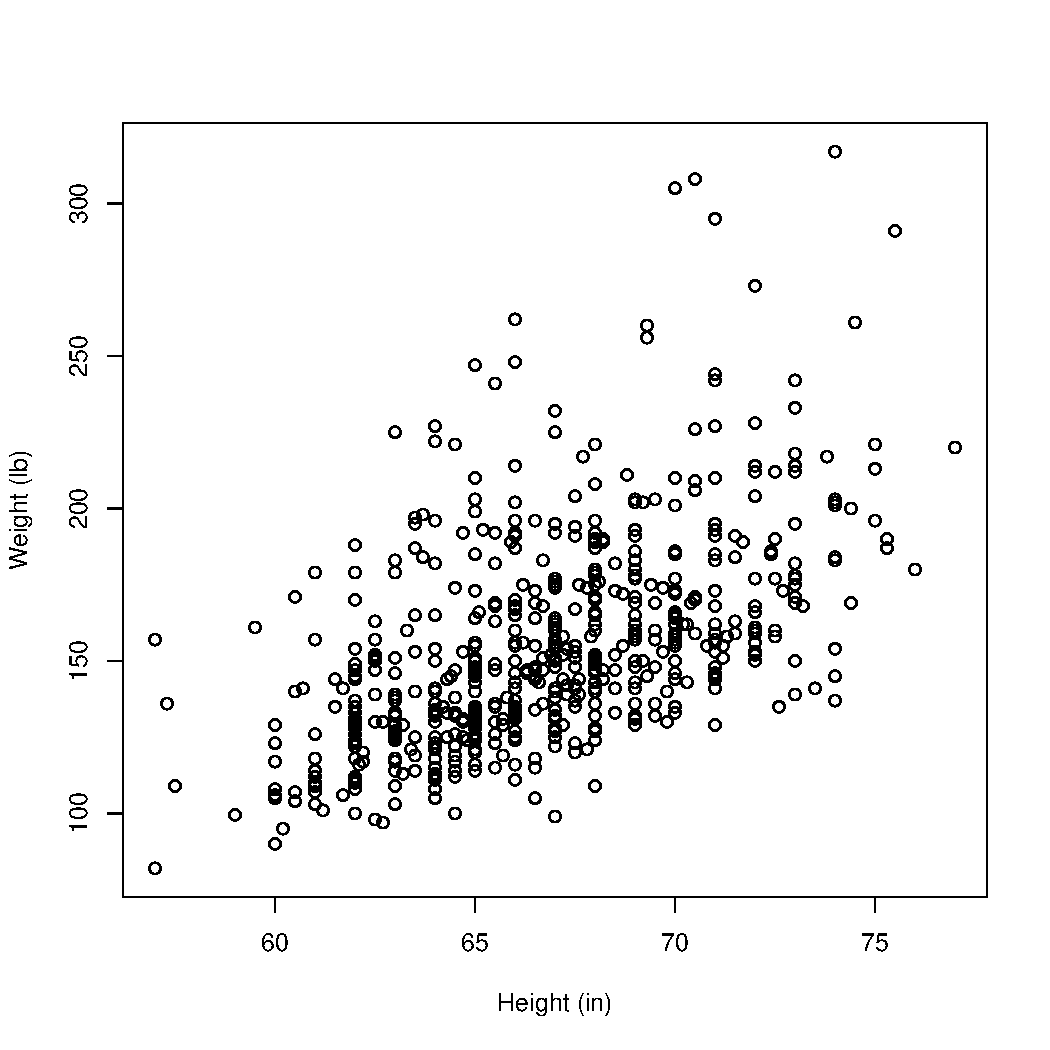
\includegraphics[width=0.45\linewidth]{figure/numerical-1} 
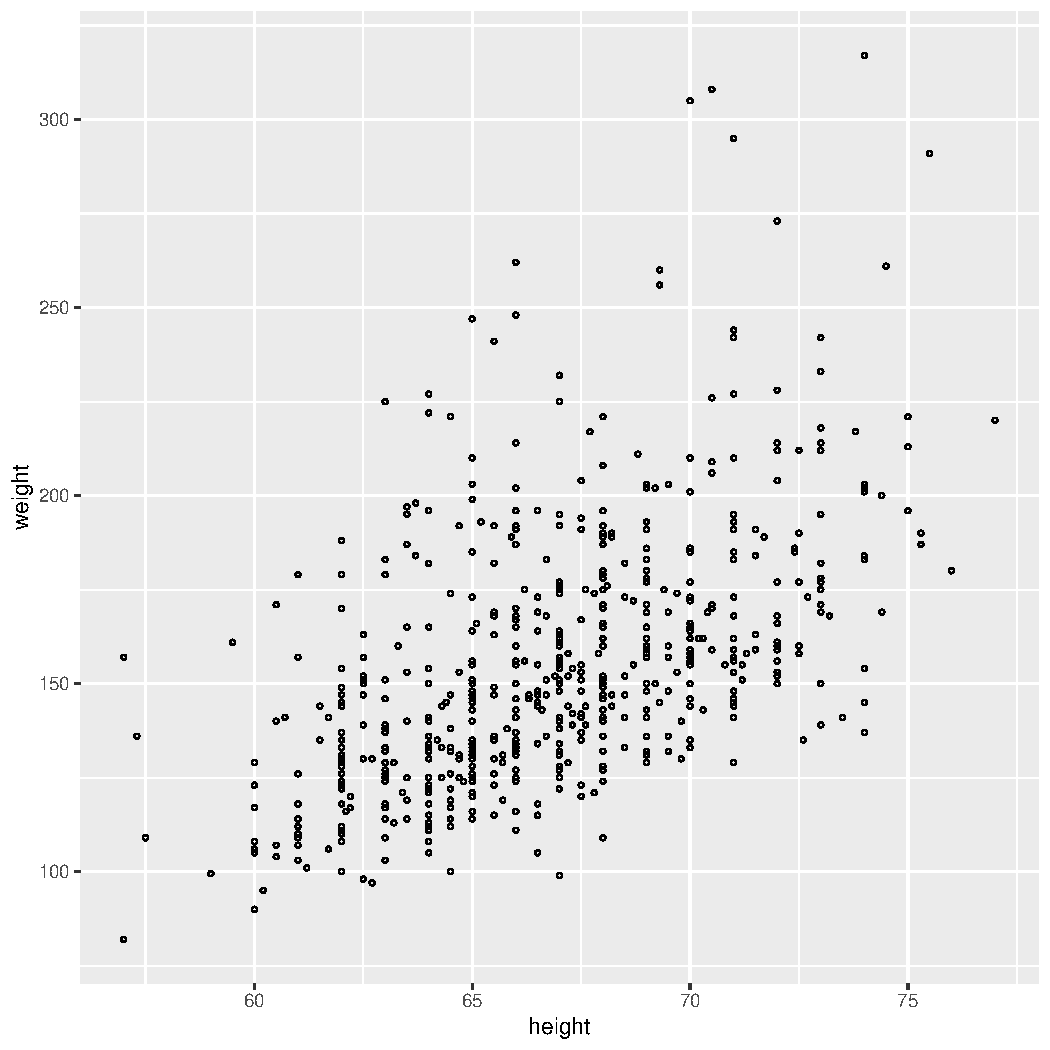
\includegraphics[width=0.45\linewidth]{figure/numerical-2} 

}



\end{knitrout}
	
	\normalsize
	
\end{frame}



						
						\begin{frame}{Pearson's correlation coefficient}
							\protect\hypertarget{two-numerical-variables}{}
							
								\begin{itemize}
							
							\item The \textbf{\textcolor{red}{sample}} correlation ($r$) between two variables $X$ and $Y$ is given by:							
							\begin{align}
							r &= \frac{1}{n-1} \sum_{i=1}^n z_X \cdot z_Y \\ 
							&=\frac{1}{n-1} \sum_{i=1}^{n}\left(\frac{x_{i}-\bar{x}}{s_{X}}\right)\left(\frac{y_{i}-\bar{y}}{s_{Y}}\right)
							\end{align}
							
							\item $\left(x_{1}, y_{1}\right),\left(x_{2}, y_{2}\right), \ldots,\left(x_{n}, y_{n}\right)$ the $n$ paired sample values of $X$ and $Y$
							
							\item $z_{X}$ and $z_{Y}$ are the sample Z-scores of the $X$ and $Y$ variables, respectively 
							
							\item $s_{X}$ and $s_{Y}$ are the sample standard deviations of the $X$ and $Y$ variables, respectively 
							
							\item $\bar{x}$ and $\bar{y}$ are the sample means of the X and Y variables, respectively
							
							
							\pause 
							
							\item The correlation coefficient quantifies the strength of a \textbf{\textcolor{red}{linear}} trend.
							
						
													\end{itemize}
							
							
						\end{frame}
						



\begin{frame}[fragile]{Plot of weight vs. height in \texttt{famuss} dataset}
	
\begin{knitrout}\tiny
\definecolor{shadecolor}{rgb}{0.969, 0.969, 0.969}\color{fgcolor}

{\centering 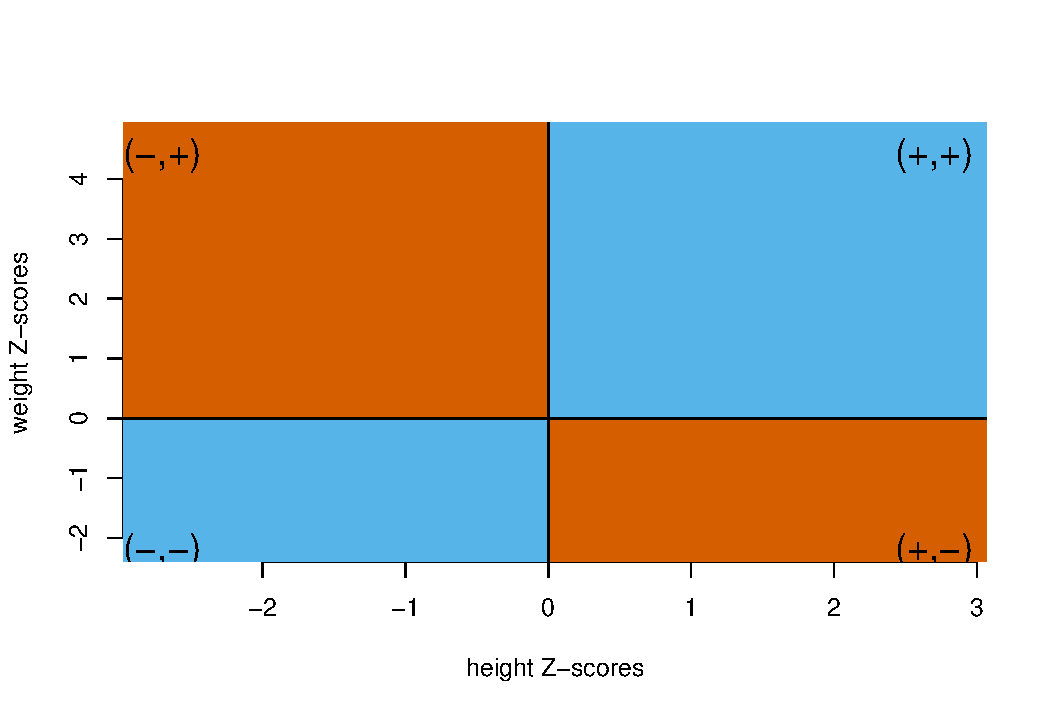
\includegraphics[width=\maxwidth]{figure/unnamed-chunk-1-1} 

}



\end{knitrout}
	
\end{frame}


\begin{frame}[fragile]{Plot of Z-scores weight vs. Z-scores height in \texttt{famuss} dataset}

\begin{knitrout}\tiny
\definecolor{shadecolor}{rgb}{0.969, 0.969, 0.969}\color{fgcolor}

{\centering 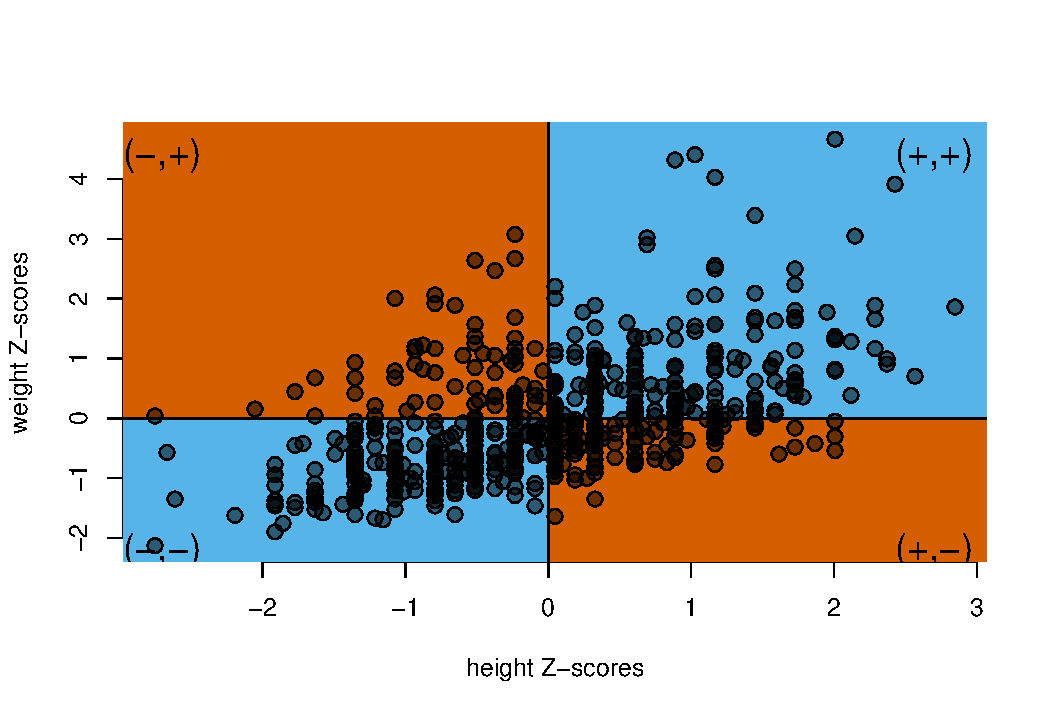
\includegraphics[width=\maxwidth]{figure/unnamed-chunk-2-1} 

}



\end{knitrout}

\end{frame}



\begin{frame}[fragile]{Partition the graph into four quadrants $(x,y)$}
	
\begin{knitrout}\tiny
\definecolor{shadecolor}{rgb}{0.969, 0.969, 0.969}\color{fgcolor}

{\centering 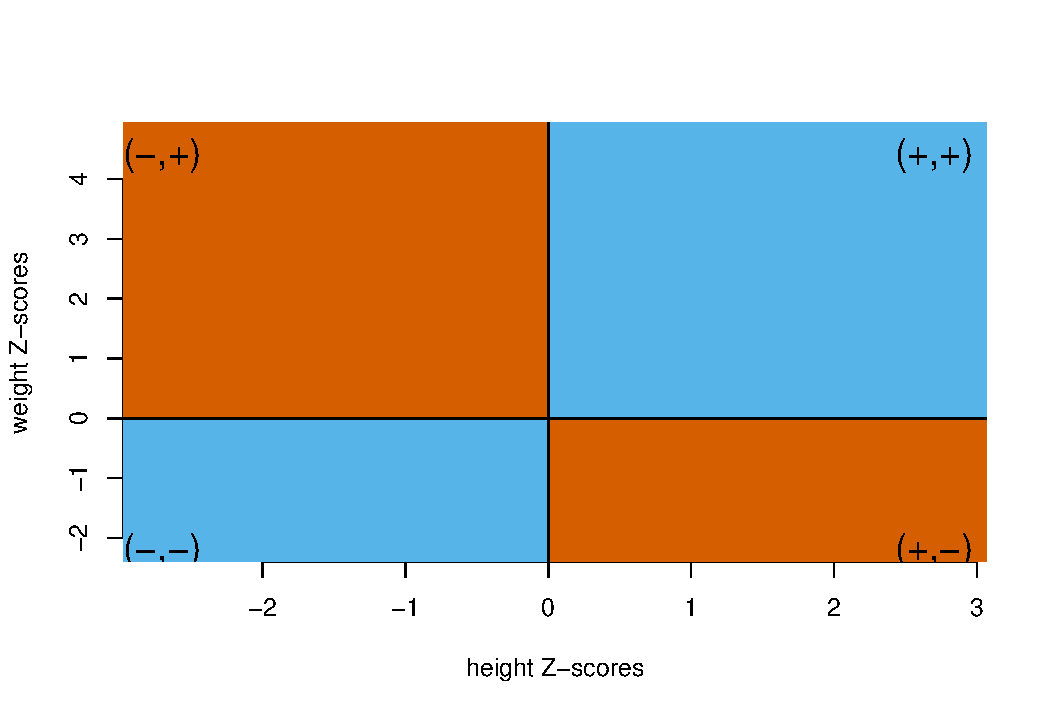
\includegraphics[width=\maxwidth]{figure/unnamed-chunk-3-1} 

}



\end{knitrout}
	
\end{frame}


\begin{frame}[fragile]{Correlation depends on which quadrants the points are on}
	
\begin{knitrout}\tiny
\definecolor{shadecolor}{rgb}{0.969, 0.969, 0.969}\color{fgcolor}

{\centering 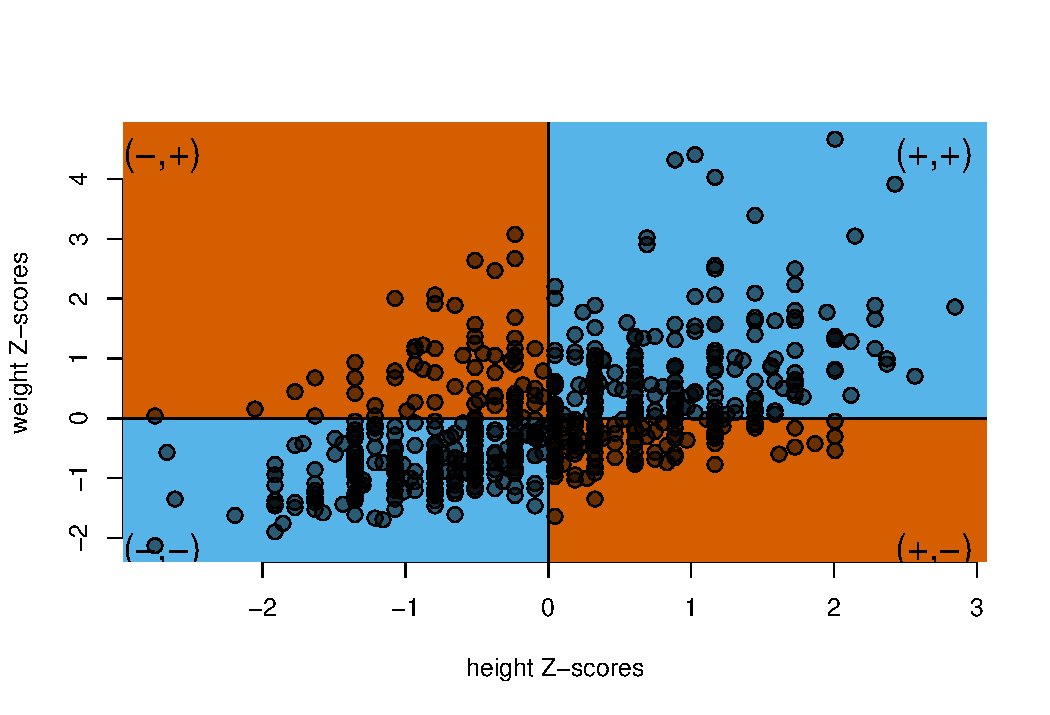
\includegraphics[width=\maxwidth]{figure/unnamed-chunk-4-1} 

}



\end{knitrout}
	
\end{frame}






						
\begin{frame}{Pearson's correlation coefficient}
	\protect\hypertarget{two-numerical-variables}{}
	
	\begin{itemize}
		
		
		\item
		The correlation coefficient \(r\) takes on values between -1 and 1.
		\pause 
		\item
		The closer \(r\) is to \(\pm 1\), the stronger the linear association.
		\pause 
		
		\item 	Two variables \(X\) and \(Y\) are
		
		\begin{itemize}
			\item
			\emph{positively associated} if \(Y\) increases as \(X\) increases ($r>0$)
			\item
			\emph{negatively associated} if \(Y\) decreases as \(X\) increases ($r<0$)
		\end{itemize}
	
	\pause 
	
	\item Since the formula for calculating the correlation coefficient standardizes the variables, changes in scale or units of measurement will not affect its value
		
	\end{itemize}
	
	
\end{frame}





\begin{frame}{Exercise: Show mathematically that the correlation ($r$) is bounded by -1 and 1}
	\pause 
	Consider that we can't have higher correlation than when we compare a list to itself (perfect correlation).
	\vspace{4in}
\end{frame}


\begin{frame}{Correlation and Simple linear Regression}
	\begin{itemize}
		\item 
If we are predicting a random variable $Y$ knowing the value of another
variable $X=x$ using a regression line, then the formula for the regression can be given by:
\begin{equation}
\left(\frac{Y-\bar{y}}{s_{Y}}\right)=r\left(\frac{x-\bar{x}}{s_{X}}\right)
\end{equation}

\item This can be rewritten as:
\begin{align}
Y &= \bar{y}+r\left(\frac{x-\bar{x}}{s_{X}}\right) s_{Y}
\end{align}

	\end{itemize}
\end{frame}








						
\begin{frame}[fragile]{Correlation in \texttt{R}}
							\protect\hypertarget{two-numerical-variables-2}{}

							\begin{itemize}							
		\item Correlation between weight and height in the \texttt{famuss} dataset:
							
						
						
\begin{knitrout}\scriptsize
\definecolor{shadecolor}{rgb}{0.969, 0.969, 0.969}\color{fgcolor}\begin{kframe}
\begin{alltt}
\hlkwd{cor}\hlstd{(famuss}\hlopt{$}\hlstd{height, famuss}\hlopt{$}\hlstd{weight)}
\end{alltt}
\begin{verbatim}
## [1] 0.53
\end{verbatim}
\end{kframe}
\end{knitrout}
							
							\pause
							
							\item We can also obtain the correlation between \texttt{weight} and \texttt{height} from a simple linear regression:
							
\begin{knitrout}\scriptsize
\definecolor{shadecolor}{rgb}{0.969, 0.969, 0.969}\color{fgcolor}\begin{kframe}
\begin{alltt}
\hlkwd{summary}\hlstd{(}\hlkwd{lm}\hlstd{(height} \hlopt{~} \hlstd{weight,} \hlkwc{data} \hlstd{= famuss))}
\end{alltt}
\begin{verbatim}
## Coefficients:
##             Estimate Std. Error t value Pr(>|t|)    
## (Intercept)  58.2952     0.5732   101.7   <2e-16 ***
## weight        0.0548     0.0036    15.2   <2e-16 ***
## ---
## Signif. codes:  0 '***' 0.001 '**' 0.01 '*' 0.05 '.' 0.1 ' ' 1
## 
## Residual standard error: 3 on 593 degrees of freedom
## Multiple R-squared: 0.282,	Adjusted R-squared: 0.281 
## F-statistic:  233 on 1 and 593 DF,  p-value: <2e-16
\end{verbatim}
\end{kframe}
\end{knitrout}
						
						\pause
						
						\item Exercise: calculate the correlation coefficient from the regression coefficient for weight. 
						
							\normalsize
							
					\end{itemize}
							
\end{frame}


\begin{frame}{Let's remind ourselves about random variability}
\begin{itemize}
	\item In many cases, we do not observe data for the entire population of interest but rather for a random sample. 
	\item As with the mean and standard deviation, the sample correlation is the most commonly used estimator of the population correlation. 
	\item This implies that the correlation we compute and use as a summary is a random variable.
\end{itemize}
\end{frame}



\begin{frame}[fragile]{Let's remind ourselves about random variability}
\small 
Lets create a pseudo population from the 595 observations by sampling \textbf{with replacement}, and calculate the correlation. Lets repeat this process 1000 times: 
\begin{knitrout}\tiny
\definecolor{shadecolor}{rgb}{0.969, 0.969, 0.969}\color{fgcolor}\begin{kframe}
\begin{alltt}
\hlstd{B} \hlkwb{<-} \hlnum{1000}\hlstd{; N} \hlkwb{<-} \hlnum{595}
\hlstd{R} \hlkwb{<-} \hlkwd{replicate}\hlstd{(B, \{}
        \hlstd{dplyr}\hlopt{::}\hlkwd{sample_n}\hlstd{(famuss,} \hlkwc{size} \hlstd{= N,} \hlkwc{replace} \hlstd{=} \hlnum{TRUE}\hlstd{)} \hlopt
        \hlstd{dplyr}\hlopt{::}\hlkwd{summarize}\hlstd{(}\hlkwc{r} \hlstd{=} \hlkwd{cor}\hlstd{(height, weight))} \hlopt
        \hlstd{dplyr}\hlopt{::}\hlkwd{pull}\hlstd{(r)}
\hlstd{\})}
\end{alltt}
\end{kframe}
\end{knitrout}

\begin{figure}
	\begin{minipage}[h]{0.30\linewidth}
\begin{knitrout}\tiny
\definecolor{shadecolor}{rgb}{0.969, 0.969, 0.969}\color{fgcolor}\begin{kframe}
\begin{alltt}
\hlkwd{mean}\hlstd{(R)}
\end{alltt}
\begin{verbatim}
## [1] 0.53
\end{verbatim}
\begin{alltt}
\hlkwd{quantile}\hlstd{(R,} \hlkwc{probs} \hlstd{=} \hlkwd{c}\hlstd{(}\hlnum{0.025}\hlstd{,} \hlnum{0.975}\hlstd{))}
\end{alltt}
\begin{verbatim}
## 2.5%  98% 
## 0.47 0.59
\end{verbatim}
\end{kframe}
\end{knitrout}
	\end{minipage}
	\hspace{0.4cm}
	\begin{minipage}[h]{0.59\linewidth}
\begin{knitrout}\tiny
\definecolor{shadecolor}{rgb}{0.969, 0.969, 0.969}\color{fgcolor}\begin{kframe}
\begin{alltt}
\hlkwd{hist}\hlstd{(R,} \hlkwc{breaks} \hlstd{=} \hlnum{20}\hlstd{,} \hlkwc{col} \hlstd{=} \hlstr{"lightblue"}\hlstd{,} \hlkwc{xlab} \hlstd{=} \hlstr{"correlation"}\hlstd{,}
     \hlkwc{main} \hlstd{=} \hlstr{"Distribution of samples of size 595"}\hlstd{)}
\hlkwd{abline}\hlstd{(}\hlkwc{v} \hlstd{=} \hlkwd{mean}\hlstd{(R),} \hlkwc{col} \hlstd{=} \hlstr{"red"}\hlstd{,} \hlkwc{lwd} \hlstd{=} \hlnum{2}\hlstd{)}
\hlkwd{abline}\hlstd{(}\hlkwc{v} \hlstd{=} \hlkwd{quantile}\hlstd{(R,} \hlkwc{probs} \hlstd{=} \hlkwd{c}\hlstd{(}\hlnum{0.025}\hlstd{,} \hlnum{0.975}\hlstd{)),} \hlkwc{col} \hlstd{=} \hlstr{"blue"}\hlstd{,}
       \hlkwc{lty} \hlstd{=} \hlnum{2}\hlstd{,} \hlkwc{lwd} \hlstd{=} \hlnum{2}\hlstd{)}
\end{alltt}
\end{kframe}

{\centering 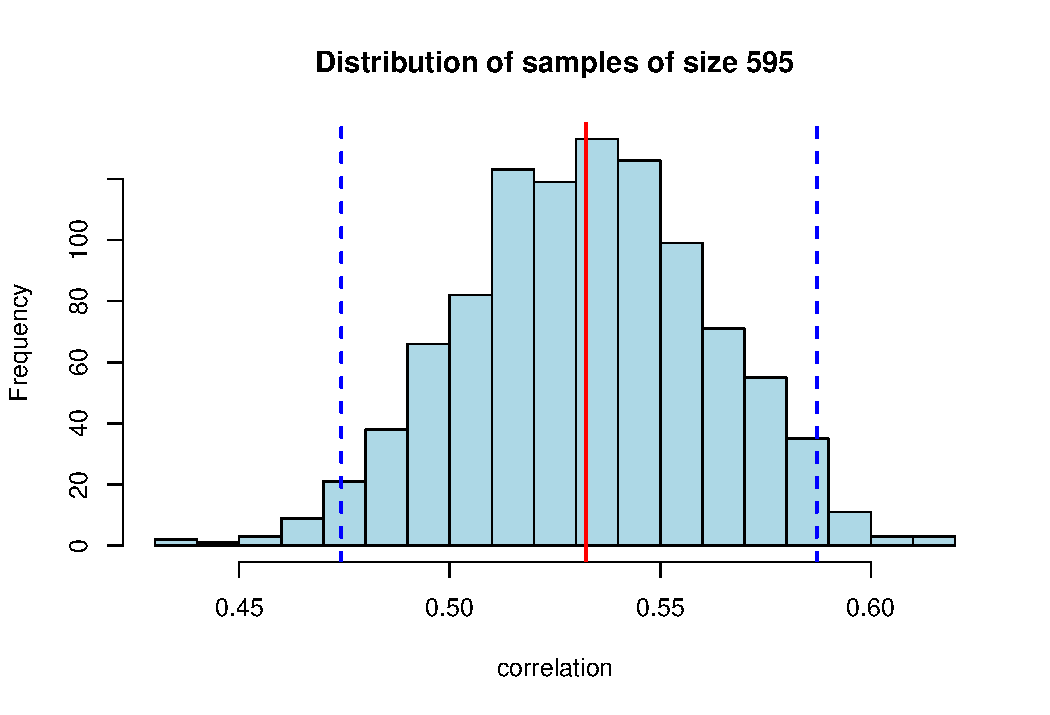
\includegraphics[width=\maxwidth]{figure/histboot-1} 

}



\end{knitrout}
	\end{minipage}
\end{figure}



\end{frame}



\begin{frame}{Another example: NHANES\footnote{\tiny{\url{http://www.cdc.gov/nchs/nhanes.htm}}}}
	\begin{itemize}
		\item The National Health and Nutrition Examination Survey (NHANES) consists of a set of surveys and measurements conducted by the US CDC to assess the health and nutritional status of adults	and children in the United States. 
		\item The following example uses data from a sample of 500 adults (individuals ages 21 and older) from the NHANES dataset\footnote{\tiny{The sample is available as \texttt{nhanes.samp.adult.500} in the \texttt{R} \code{oibiostat} package}}.
	\end{itemize}
\end{frame}

\begin{frame}[fragile,plain]

\vspace{-0.5in}	
	
\begin{knitrout}\tiny
\definecolor{shadecolor}{rgb}{0.969, 0.969, 0.969}\color{fgcolor}\begin{figure}

{\centering \subfloat[\label{fig:unnamed-chunk-6-1}]{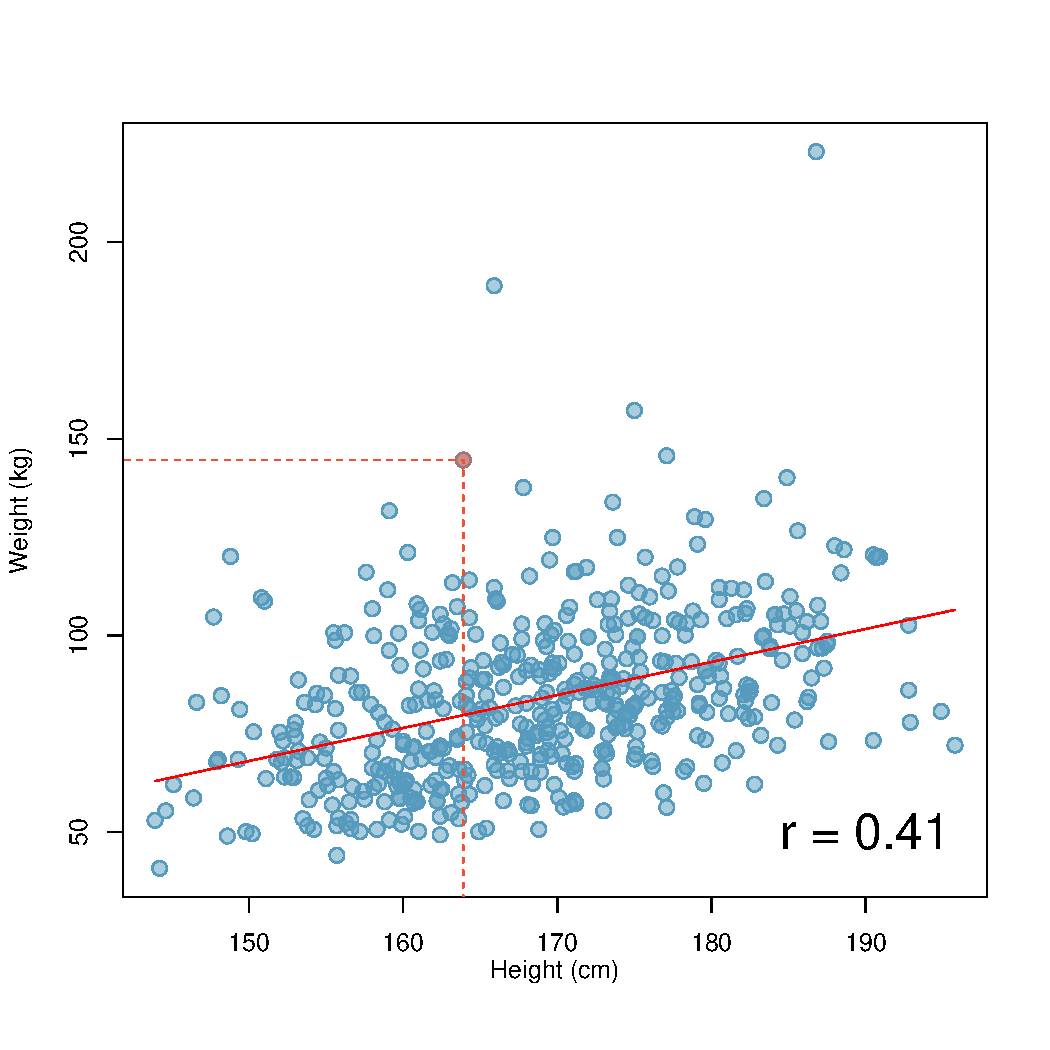
\includegraphics[width=0.55\linewidth]{figure/unnamed-chunk-6-1} }
\subfloat[\label{fig:unnamed-chunk-6-2}]{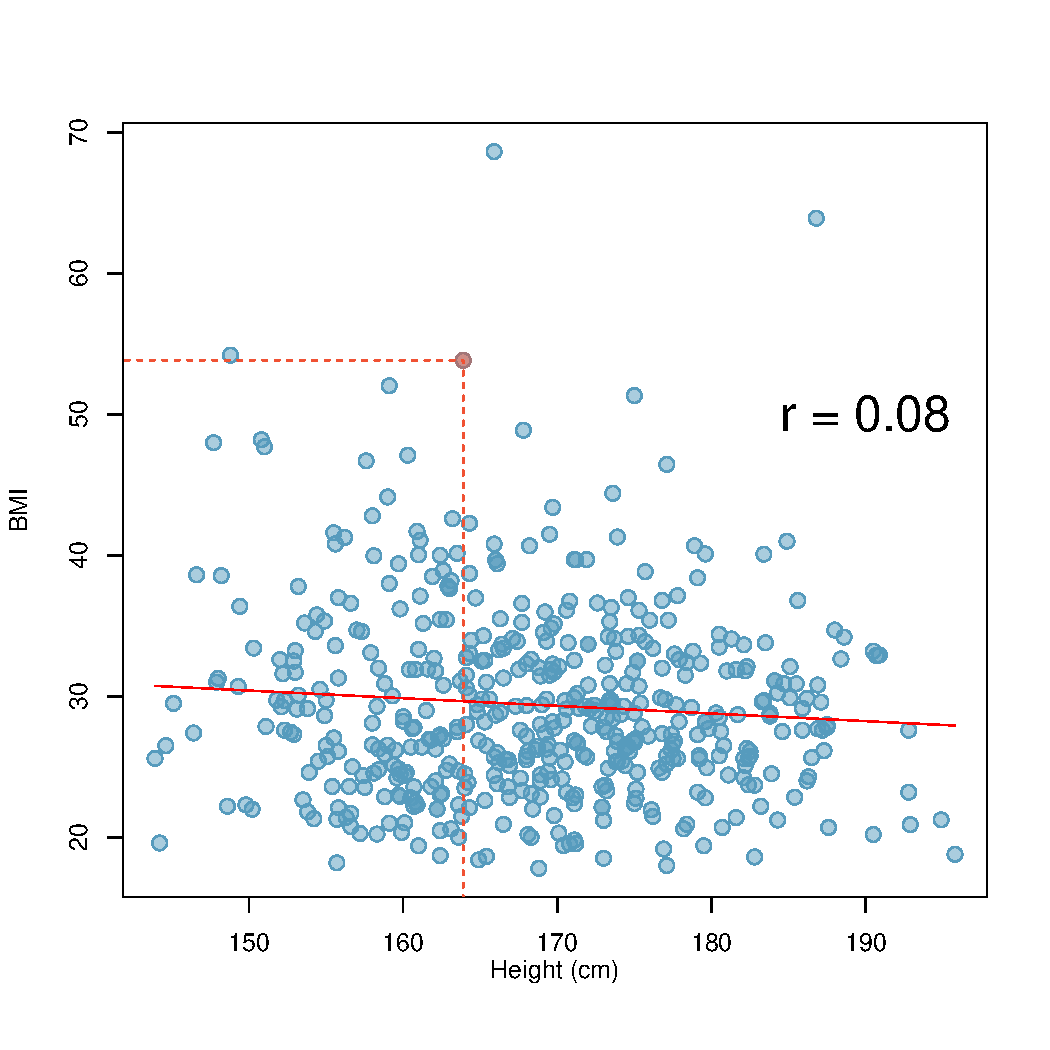
\includegraphics[width=0.55\linewidth]{figure/unnamed-chunk-6-2} }

}

\caption[(a) A scatterplot showing height versus weight from the 500 individuals in the sample from NHANES]{(a) A scatterplot showing height versus weight from the 500 individuals in the sample from NHANES. One participant 163.9 cm tall (about 5 ft, 4 in) and weighing 144.6 kg (about 319 lb) is highlighted. (b) A scatterplot showing height versus BMI from the 500 individuals in the sample from NHANES. The same individual highlighted in (a) is marked here, with BMI 53.83. Fitted regression lines are shown in red with correlation coefficient $r$. BMI = weight/height$^2$ $\times 703$.}\label{fig:unnamed-chunk-6}
\end{figure}


\end{knitrout}
	
\end{frame}




\frame{\frametitle{Cautionary notes}
	\begin{itemize}
		
		\item The formulas above are for a \underline{particular sample}, hence the lower case letters $r,x,y$. In statistical terms, $r$ is the \textbf{estimator} for the population-level correlation $\rho$ (the \textbf{estimand}) of the random variables $X$ and $Y$. The actual value of the sample correlation is denoted by $\widehat{r}$ and is called the \textbf{estimate}
		
		\pause
		
	
		\item This implies that we are not 100\% confident in our estimate and therefore should provide a confidence interval  as well.
		
		\pause
		

		
		\item A strong linear relationship is not necessarily a
		\textbf{causal} relationship, that is, just because $r \approx 1$ (or $r \approx -1$)
		does not mean that $x$ \textbf{causes} changes in $y$ (we may have a \textit{spurious}
		correlation).  \pause
		
		
		
		\item Just because $r \approx 0$ does not mean that that $x$ and $y$
		are unrelated, merely that they are \textbf{uncorrelated}. That
		is, it is possible to construct examples where $x$ and $y$ have
		a strong functional relationship, but where $r=0$.
		
		\item $X,Y$ independent $\Rightarrow$ $r_{XY} = 0$
		\item $r_{XY} = 0$ $\not \Rightarrow$ $X,Y$ are independent
		
	\end{itemize}


	
}





\begin{frame}[fragile]{Anscombe's quartet\footnote{\tiny{Anscombe, Francis J. (1973). Graphs in statistical analysis. The American Statistician, 27, 17–21. doi: 10.2307/2682899.}}}
	
\begin{knitrout}\tiny
\definecolor{shadecolor}{rgb}{0.969, 0.969, 0.969}\color{fgcolor}\begin{kframe}
\begin{alltt}
\hlkwd{library}\hlstd{(datasets);}\hlkwd{data}\hlstd{(}\hlstr{"anscombe"}\hlstd{)}
\end{alltt}
\end{kframe}\begin{figure}

{\centering 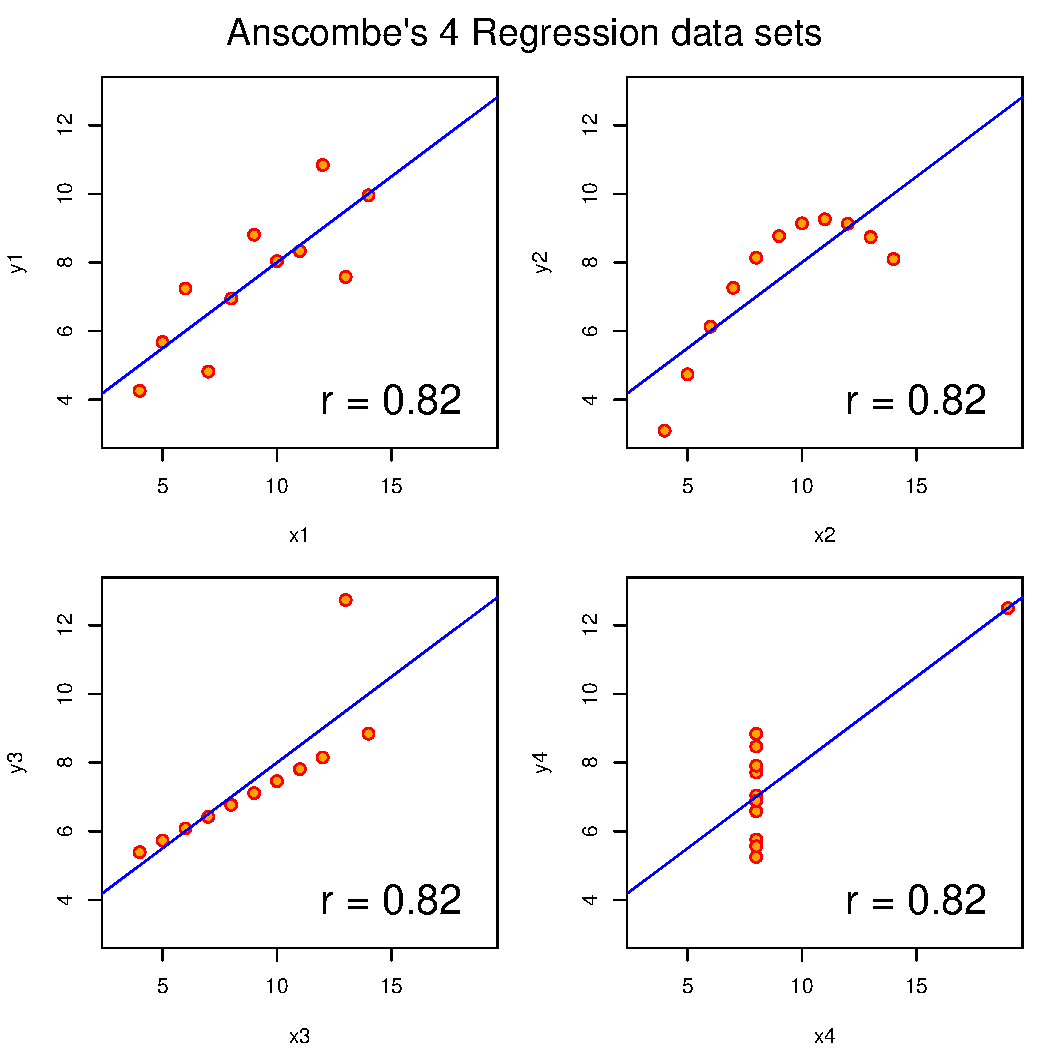
\includegraphics[width=0.55\linewidth]{figure/unnamed-chunk-7-1} 

}

\caption[All four panels have the exact same linear correlation coefficient]{All four panels have the exact same linear correlation coefficient}\label{fig:unnamed-chunk-7}
\end{figure}


\end{knitrout}


\end{frame}



\begin{frame}[fragile]{Zero linear correlation does not imply independence}
\begin{knitrout}\scriptsize
\definecolor{shadecolor}{rgb}{0.969, 0.969, 0.969}\color{fgcolor}\begin{kframe}
\begin{alltt}
\hlkwd{set.seed}\hlstd{(}\hlnum{12}\hlstd{)}
\hlstd{x} \hlkwb{<-} \hlkwd{runif}\hlstd{(}\hlnum{100}\hlstd{,}\hlopt{-}\hlnum{1}\hlstd{,}\hlnum{1}\hlstd{)}
\hlstd{y} \hlkwb{<-} \hlstd{x}\hlopt{^}\hlnum{2}
\hlkwd{plot}\hlstd{(x,y,} \hlkwc{pch} \hlstd{=} \hlnum{19}\hlstd{)}
\end{alltt}
\end{kframe}

{\centering 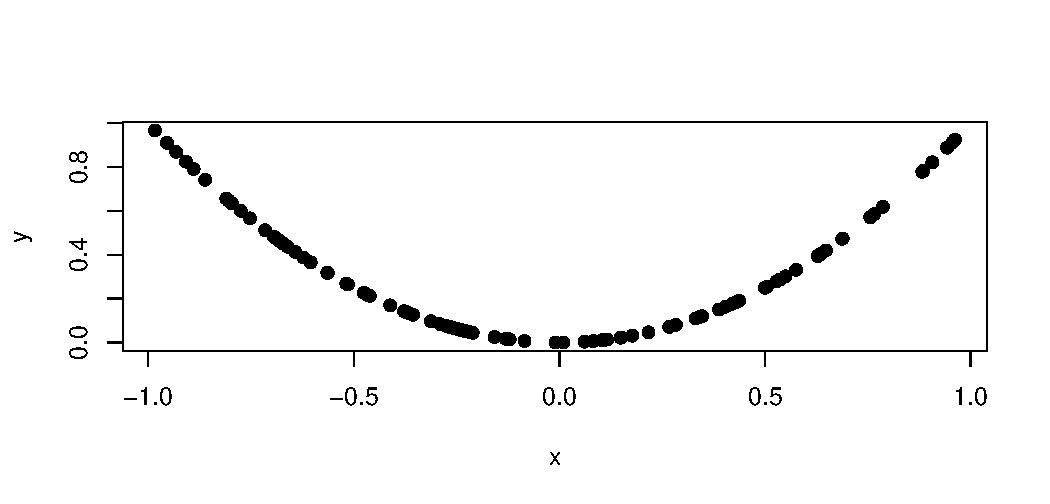
\includegraphics[width=\maxwidth]{figure/unnamed-chunk-8-1} 

}


\begin{kframe}\begin{alltt}
\hlkwd{cor}\hlstd{(x,y)}
\end{alltt}
\begin{verbatim}
## [1] -0.023
\end{verbatim}
\end{kframe}
\end{knitrout}
\end{frame}


\begin{frame}{Another example of same summary statistics but very different relationships}
\url{https://www.autodeskresearch.com/publications/samestats}
\end{frame}




\begin{frame}[fragile,plain]{Transformations to improve linear fit}
	
\begin{knitrout}\tiny
\definecolor{shadecolor}{rgb}{0.969, 0.969, 0.969}\color{fgcolor}\begin{figure}

{\centering \subfloat[\label{fig:004-nyt-1}]{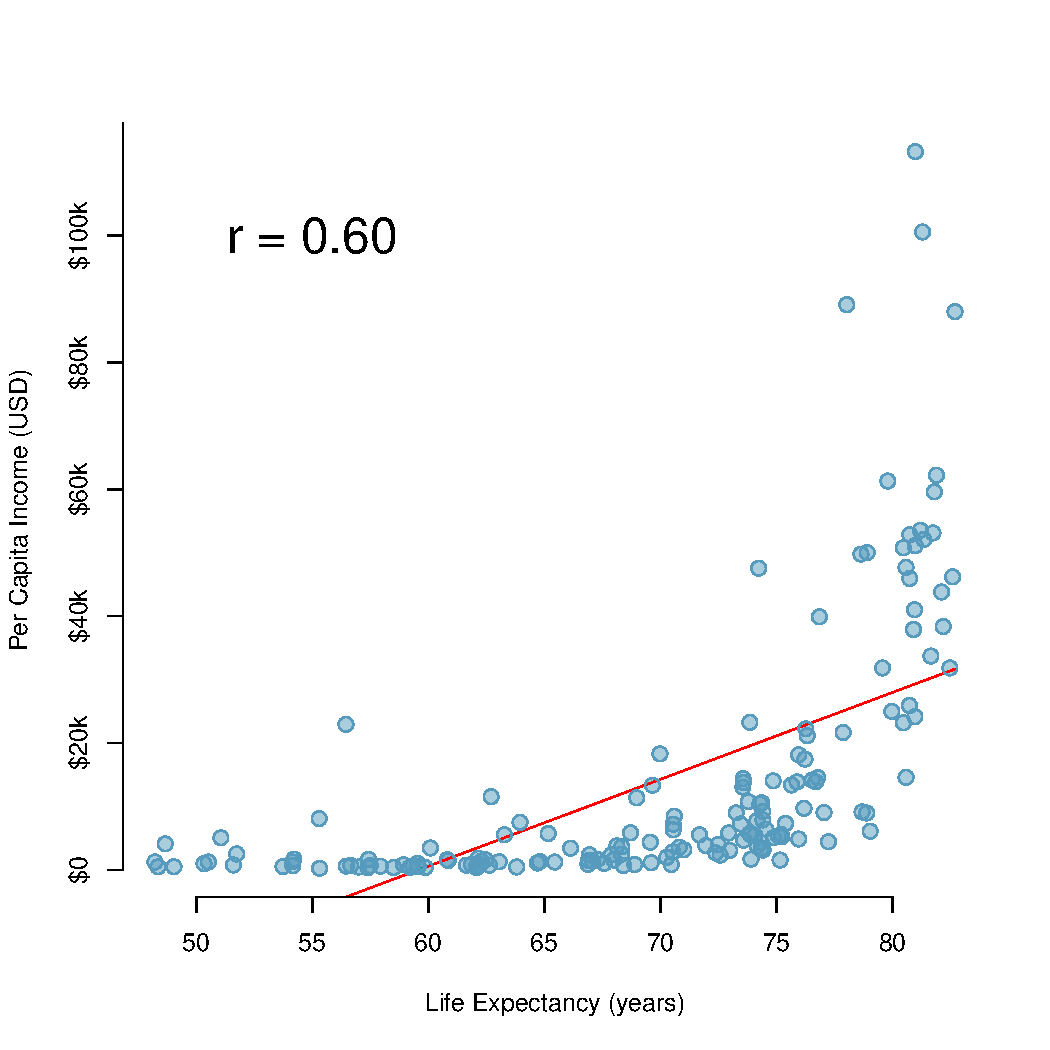
\includegraphics[width=0.53\linewidth]{figure/004-nyt-1} }
\subfloat[\label{fig:004-nyt-2}]{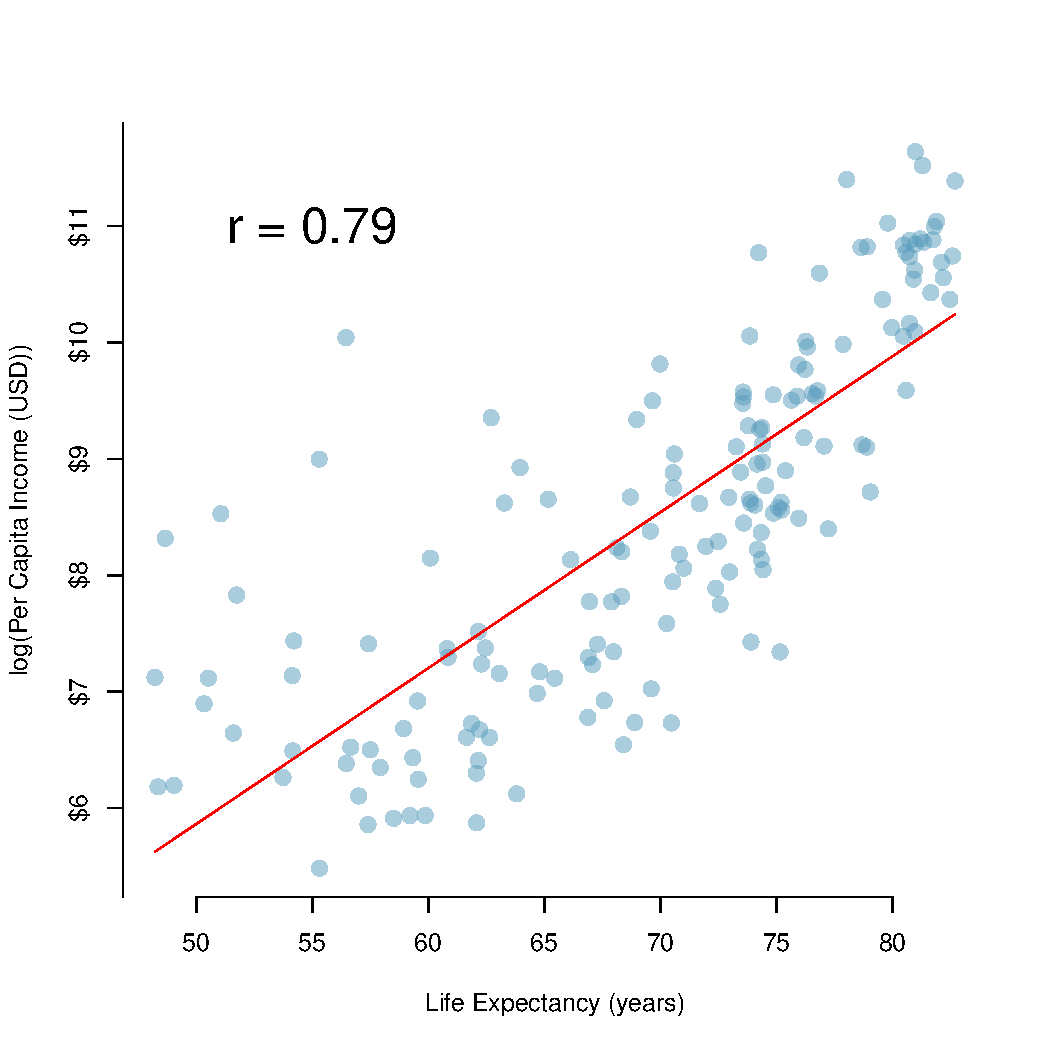
\includegraphics[width=0.53\linewidth]{figure/004-nyt-2} }

}

\caption{(a) per capita income vs. life expectancy (b) log per capita income vs. life expectancy. Fitted regression line in red with correlation coefficient $r$.\footnote{\tiny{The World Development Indicators (WDI) is a database of country-level variables (i.e., indicators) recording outcomes for a variety of topics, including economics, health, mortality, fertility, and education}}}\label{fig:004-nyt}
\end{figure}


\end{knitrout}
	
\end{frame}



\frame{\frametitle{Rank correlation} The Pearson correlation,
	recall, is a measure of \textit{linear} association. This may
	be undesirable for a number of reasons:
	\begin{itemize}
		\item $y$ and $x$ may be related, but not linearly (e.g., shape
		may be quadratic) \pause
		\item one or both of $y$ and $x$ may be an ordered categorical
		variable (e.g., highest level of education attained, income category, age group, etc.)
		and the investigator may not wish to impose a particular numerical scale \pause
		\item A nonparametric approach may be preferred if $y$ or $x$
		are thought not to be Normally distributed
	\end{itemize}
	We can overcome these concerns using a correlation that is
	based on the ranks of the data, called \textbf{Spearman's rank
		correlation}. } \frame{\frametitle{Spearman's rank correlation}
	This is most easily understood through the use of an example. \\ \ \\
	
	Suppose we want to examine the correlation between gestational
	age (GA) and birthweight (BW). {\footnotesize
		\begin{center}
			\begin{tabular}{|l|cccccccc|} \hline
				Infant & 1&2&3&4&5&6&7&8 \\ \hline
				BW (g) &2621&2863&3322&3508&3518&3770&3784&3801 \\
				GA (days) &270&271&267&268&276&282&288&278 \\
				\hline
				BW rank &1&2&3&4&5&6&7&8 \\
				GA rank &3&4&1&2&5&7&8&6 \\ \hline
			\end{tabular}
	\end{center} }
} \frame{\frametitle{Spearman's rank correlation} Spearman's
	rank correlation is based on the squared differences in rank
	for each individual:
	\begin{center}
		\begin{tabular}{|l|cccccccc|} \hline
			Infant & 1&2&3&4&5&6&7&8 \\ \hline
			Rank by BW &1&2&3&4&5&6&7&8 \\
			Rank by GA &3&4&1&2&5&7&8&6 \\ \hline
			Difference &-2&-2&2&2&0&-1&-1&2 \\
			Difference$^2$ &4&4&4&4&0&1&1&4 \\ \hline
		\end{tabular}
	\end{center}
	
	Then Spearman's rank correlation coefficient is computed to be
	\[ r_s = 1- \frac{6\sum d^2}{n^3-n}\]
	
	In our example, this gives $r_s = 0.738$. }

\frame{\frametitle{Spearman's rank correlation} Spearman's rank
	correlation is equivalent to calculating a Pearson's
	correlation on the ranks:
	\[r = \hbox{Corr}(\hbox{Rank}_{\hbox{GA}},\hbox{Rank}_{\hbox{BW}}) = 0.738 \]
}

\frame{\frametitle{Rank correlation: Kendall's $\tau$} There is
	another rank correlation, Kendall's $\tau$, which we will again
	learn by example. \\ \ \\
	
	We study the correlation between gestational age and
	birthweight. {\footnotesize
		\begin{center}
			\begin{tabular}{|l|cccccccc|} \hline
				Infant & 1&2&3&4&5&6&7&8 \\ \hline
				BW (g) &2621&2863&3322&3508&3518&3770&3784&3801 \\
				GA (days) &270&271&267&268&276&282&288&278 \\
				\hline
				BW rank&1&2&3&4&5&6&7&8 \\
				GA rank &3&4&1&2&5&7&8&6 \\ \hline
			\end{tabular}
	\end{center} }
	
} \frame{\frametitle{Rank correlation: Kendall's $\tau$}
	\begin{center}
		\begin{tabular}{|l|cccccccc|} \hline
			Infant & 1&2&3&4&5&6&7&8 \\ \hline
			Rank by b.weight &1&2&3&4&5&6&7&8 \\
			Rank by gest.age &3&4&1&2&5&7&8&6 \\ \hline
		\end{tabular}
	\end{center}
	First, we order the data according to one of the rankings (we
	chose to do so with birthweight).\\ \ \\
	
	Next, we sum the number of infants to the right of each cell
	with a \textbf{higher} ranking for the \textit{other} variable
	(gestational age), and call this $P$:
	\[P = 5+4+5+4+3+1+0=22\]
} \frame{\frametitle{Rank correlation: Kendall's $\tau$}
	
	Then Kendall's rank correlation coefficient is computed to be
	\[ \tau = \frac{2\times P}{\frac{1}{2}n(n-1)}-1\]
	
	In our example, this gives $\tau = 0.57$. \\ \ \\ \ \\ \pause
	
	We can perform hypothesis testing on Kendall's $\tau$; the
	approximately Normal test statistic is \[z = \frac{2\times
		P}{\sqrt{n(n-1)(2n+5)/18}}\] } \frame{\frametitle{Rank
		correlation: Kendall's $\tau$} In our example, if we wish to
	test $H_0: \tau=0$ vs.~$H_A: \tau \ne 0$, this gives
	\begin{eqnarray*}
		z & = & \frac{2\times P}{\sqrt{n(n-1)(2n+5)/18}}\\
		& = & \frac{2\times 22}{\sqrt{8\times7\times21/18}}\\
		& = & 5.444
	\end{eqnarray*}
	which yields a p-value of $P(|Z|>5.444) < 0.001$, indicating
	that there is a statistically significant association as
	measured by Kendall's rank correlation between gestational age
	and birthweight. }

\frame{\frametitle{Rank correlation} \textbf{Notes:}\\
	\begin{itemize}
		\item Both Spearman's and Kendall's correlations lie between
		$-1$ and 1; positive values correspond to a positive association, negative values to a
		negative association. \pause
		\item Both Spearman's and Kendall's correlations are
		nonparametric statistics. \pause
		\item Corrections for ties are required (beyond the scope of this course). \texttt{R} handles it for you.
	\end{itemize}
	
}
			

						
\section{Two categorical variables and contingency tables}
						
\begin{frame}[fragile]{Two categorical variables}
A contingency table summarizes data for two categorical variables:
\begin{knitrout}\scriptsize
\definecolor{shadecolor}{rgb}{0.969, 0.969, 0.969}\color{fgcolor}\begin{kframe}
\begin{alltt}
\hlstd{tab1} \hlkwb{<-} \hlkwd{table}\hlstd{(famuss}\hlopt{$}\hlstd{race,}
              \hlstd{famuss}\hlopt{$}\hlstd{actn3.r577x)}
\hlstd{tab1}
\end{alltt}
\begin{verbatim}
##             
##               CC  CT  TT
##   African Am  16   6   5
##   Asian       21  18  16
##   Caucasian  125 216 126
##   Hispanic     4  10   9
##   Other        7  11   5
\end{verbatim}
\begin{alltt}
\hlkwd{addmargins}\hlstd{(tab1)}
\end{alltt}
\begin{verbatim}
##             
##               CC  CT  TT Sum
##   African Am  16   6   5  27
##   Asian       21  18  16  55
##   Caucasian  125 216 126 467
##   Hispanic     4  10   9  23
##   Other        7  11   5  23
##   Sum        173 261 161 595
\end{verbatim}
\end{kframe}
\end{knitrout}
\end{frame}
					
					
					
					
\begin{frame}[fragile]{Conditional distribution of genotype \textit{given} race}
\begin{figure}
\begin{minipage}[h]{0.30\linewidth}
\small 
			\begin{center}
			The distributions we create this way are called \textbf{\textcolor{blue}{conditional distributions}}, because they show the distribution of one variable for just those cases that satisfy a condition on another variable
			\end{center}

\normalsize
\begin{knitrout}\tiny
\definecolor{shadecolor}{rgb}{0.969, 0.969, 0.969}\color{fgcolor}\begin{kframe}
\begin{alltt}
\hlkwd{addmargins}\hlstd{(}
  \hlkwd{prop.table}\hlstd{(tab1,} \hlkwc{margin} \hlstd{=} \hlnum{1}\hlstd{)}
\hlstd{)}
\end{alltt}
\begin{verbatim}
##             
##                CC   CT   TT  Sum
##   African Am 0.59 0.22 0.19 1.00
##   Asian      0.38 0.33 0.29 1.00
##   Caucasian  0.27 0.46 0.27 1.00
##   Hispanic   0.17 0.43 0.39 1.00
##   Other      0.30 0.48 0.22 1.00
##   Sum        1.72 1.93 1.35 5.00
\end{verbatim}
\end{kframe}
\end{knitrout}
\end{minipage}
\hspace{0.4cm}
\begin{minipage}[h]{0.59\linewidth}


\begin{knitrout}\tiny
\definecolor{shadecolor}{rgb}{0.969, 0.969, 0.969}\color{fgcolor}\begin{kframe}
\begin{alltt}
\hlstd{sjPlot}\hlopt{::}\hlkwd{plot_xtab}\hlstd{(famuss}\hlopt{$}\hlstd{race,}
                  \hlstd{famuss}\hlopt{$}\hlstd{actn3.r577x,}
                  \hlkwc{margin} \hlstd{=} \hlstr{"row"}\hlstd{)}
\end{alltt}
\end{kframe}

{\centering 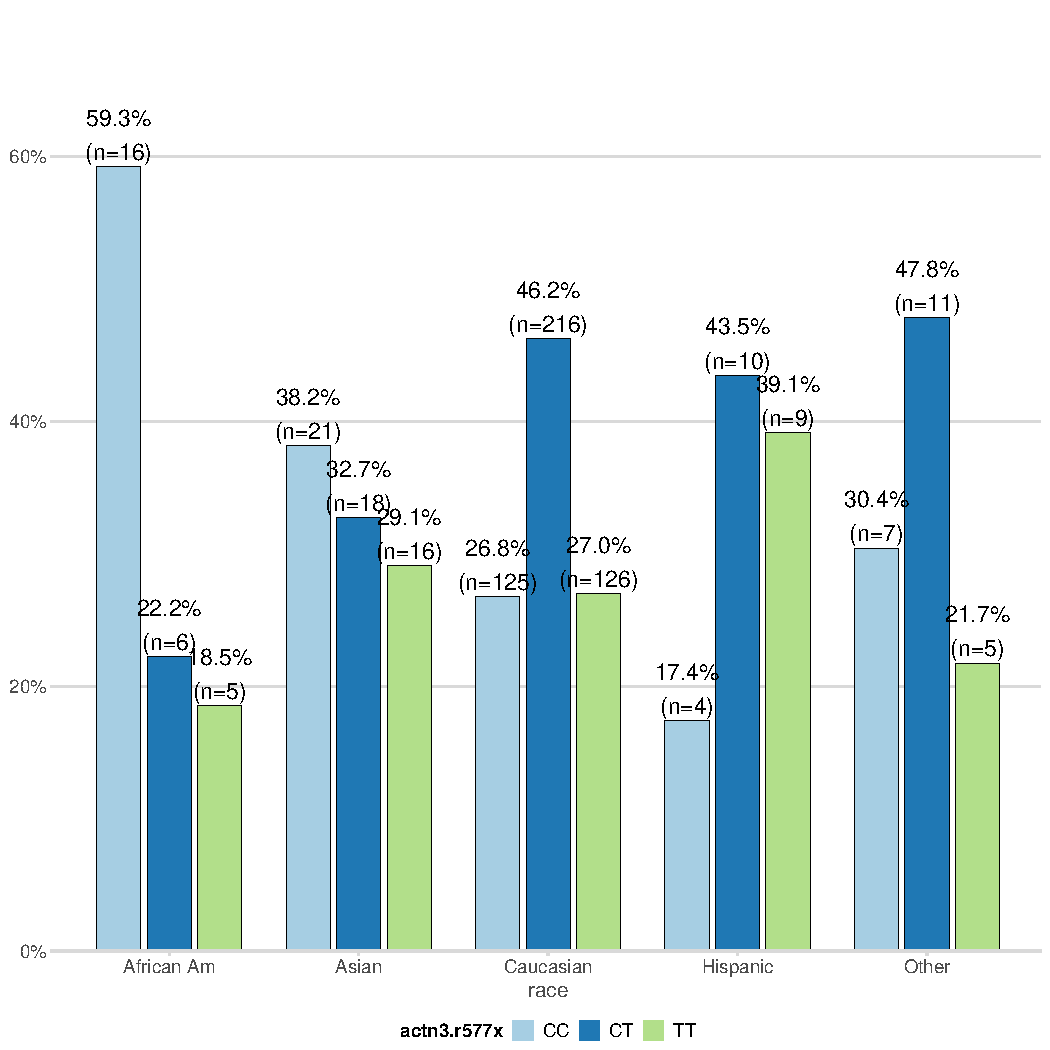
\includegraphics[width=\maxwidth]{figure/genotype-marginals-1} 

}



\end{knitrout}
\end{minipage}
\end{figure}
\end{frame}
	
\begin{frame}[fragile]{Conditional distribution of race \textit{given} genotype}

\begin{knitrout}\tiny
\definecolor{shadecolor}{rgb}{0.969, 0.969, 0.969}\color{fgcolor}\begin{kframe}
\begin{alltt}
\hlkwd{addmargins}\hlstd{(}\hlkwd{prop.table}\hlstd{(tab1,} \hlkwc{margin} \hlstd{=} \hlnum{2}\hlstd{))}
\end{alltt}
\begin{verbatim}
##             
##                 CC    CT    TT   Sum
##   African Am 0.092 0.023 0.031 0.147
##   Asian      0.121 0.069 0.099 0.290
##   Caucasian  0.723 0.828 0.783 2.333
##   Hispanic   0.023 0.038 0.056 0.117
##   Other      0.040 0.042 0.031 0.114
##   Sum        1.000 1.000 1.000 3.000
\end{verbatim}
\end{kframe}
\end{knitrout}

\begin{knitrout}\tiny
\definecolor{shadecolor}{rgb}{0.969, 0.969, 0.969}\color{fgcolor}\begin{kframe}
\begin{alltt}
\hlstd{sjPlot}\hlopt{::}\hlkwd{plot_xtab}\hlstd{(famuss}\hlopt{$}\hlstd{race, famuss}\hlopt{$}\hlstd{actn3.r577x,} \hlkwc{margin} \hlstd{=} \hlstr{"col"}\hlstd{,} \hlkwc{show.total} \hlstd{= F,} \hlkwc{show.n} \hlstd{= F)}
\end{alltt}
\end{kframe}

{\centering 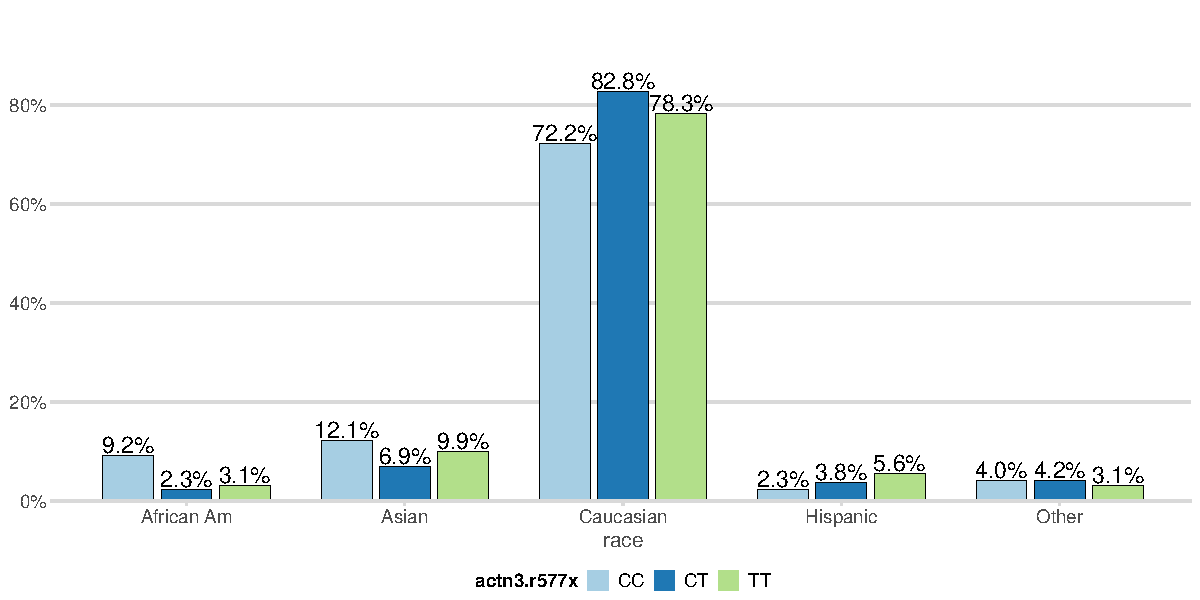
\includegraphics[width=\maxwidth]{figure/race-marginals-1} 

}



\end{knitrout}

\end{frame}

\begin{frame}[fragile]{Marginal distributions of race and genotype}
Given a contingency table, the frequency distribution of one of the variables is called its \textcolor{blue}{\textbf{marginal distribution}}.

\begin{knitrout}\tiny
\definecolor{shadecolor}{rgb}{0.969, 0.969, 0.969}\color{fgcolor}\begin{kframe}
\begin{alltt}
\hlkwd{table}\hlstd{(famuss}\hlopt{$}\hlstd{race)} \hlopt{/} \hlkwd{nrow}\hlstd{(famuss)}
\end{alltt}
\begin{verbatim}
## 
## African Am      Asian  Caucasian   Hispanic      Other 
##      0.045      0.092      0.785      0.039      0.039
\end{verbatim}
\begin{alltt}
\hlstd{sjPlot}\hlopt{::}\hlkwd{plot_frq}\hlstd{(famuss}\hlopt{$}\hlstd{race)}
\hlstd{sjPlot}\hlopt{::}\hlkwd{plot_frq}\hlstd{(famuss}\hlopt{$}\hlstd{actn3.r577x)}
\end{alltt}
\end{kframe}

{\centering 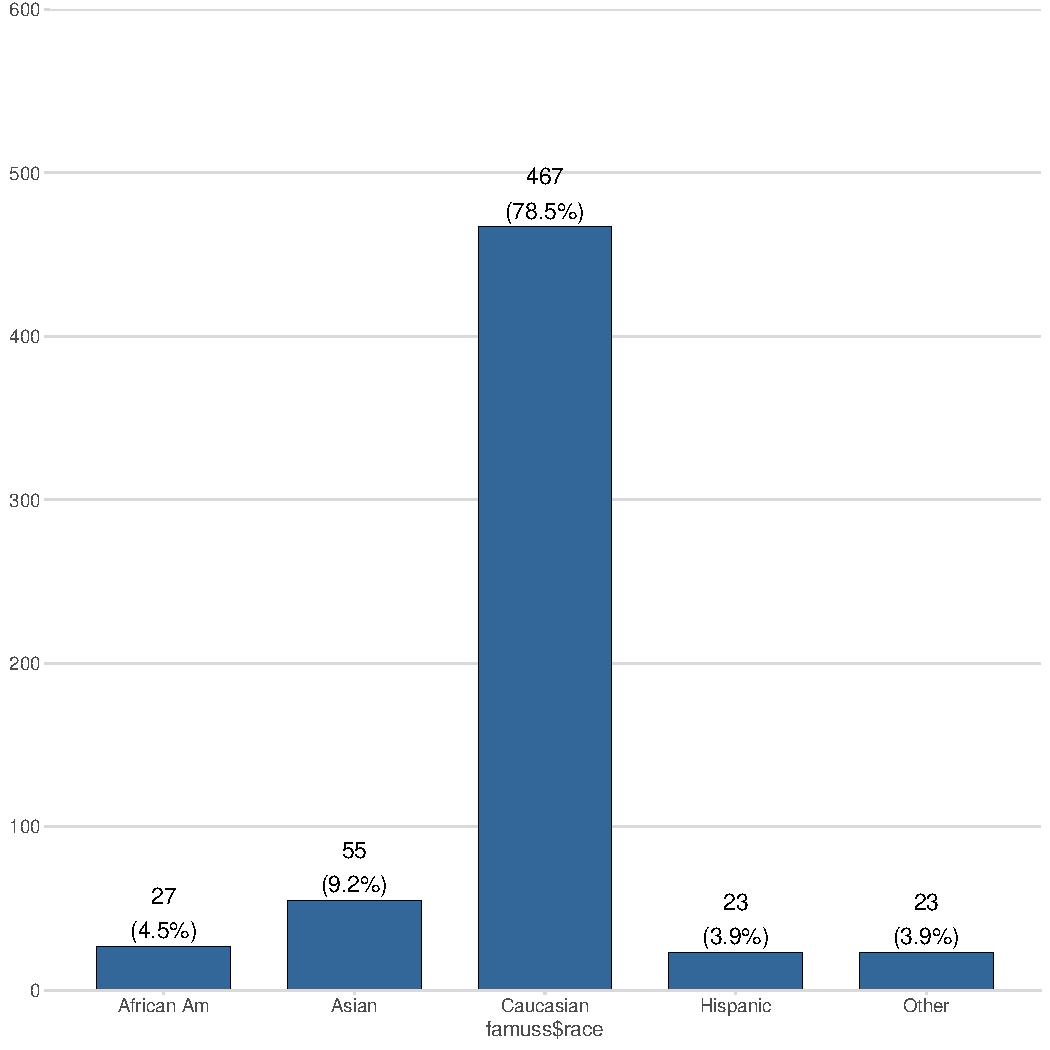
\includegraphics[width=0.45\linewidth]{figure/unnamed-chunk-10-1} 
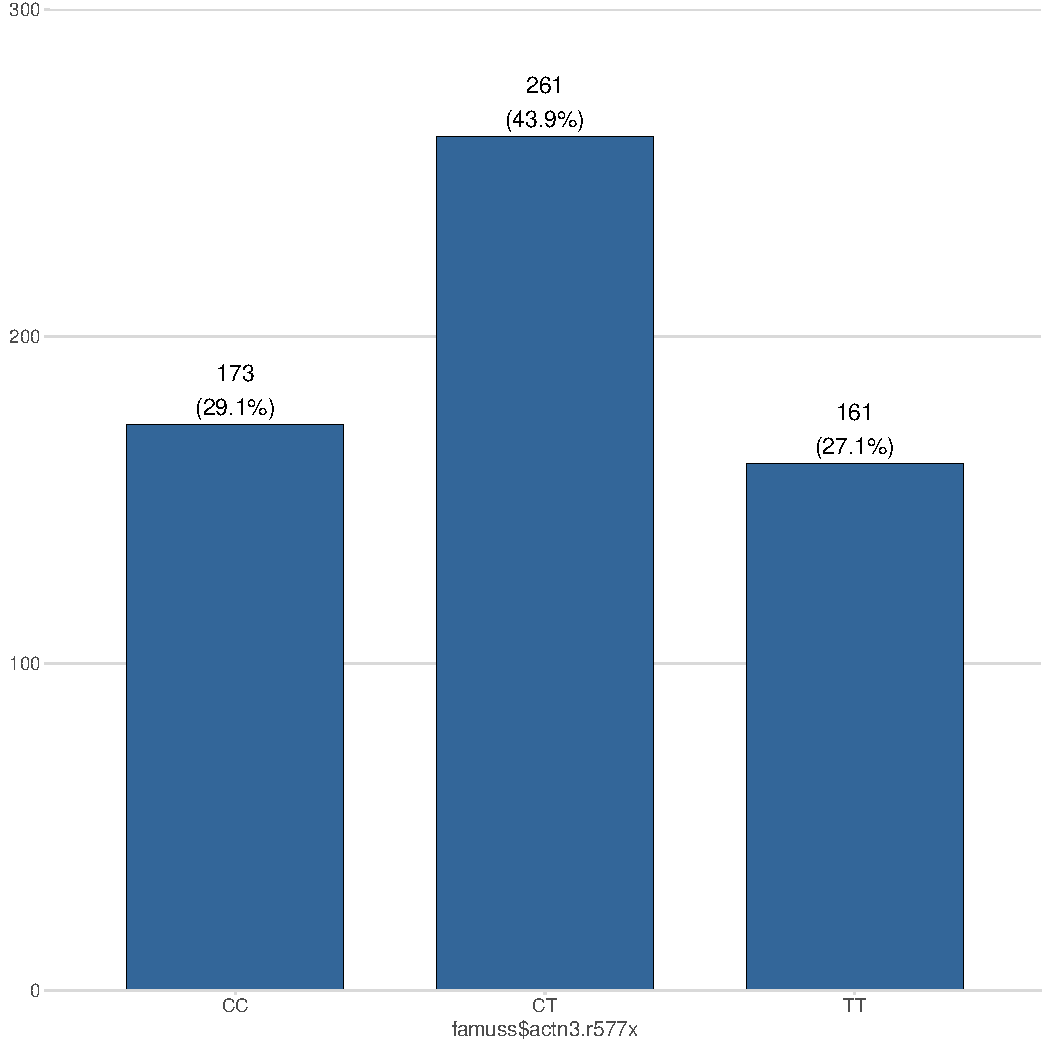
\includegraphics[width=0.45\linewidth]{figure/unnamed-chunk-10-2} 

}



\end{knitrout}

\end{frame}



\begin{frame}{Mosaic plots}
%	\small
\begin{itemize}
	\item A mosaic plot is a graphical display that allows you to examine the relationship among two or more categorical variables.
	\item The mosaic plot starts as a square with length one. The square is divided first into horizontal bars whose widths are proportional to the probabilities associated with the first categorical variable. 
	\item Then each bar is split vertically into bars that are proportional to the conditional probabilities of the second categorical
	variable. Additional splits can be made if wanted using a third, fourth variable, etc.
\end{itemize}

\end{frame}

\begin{frame}[fragile]{Mosaic plots - race and genotype}
	

	
\begin{knitrout}\tiny
\definecolor{shadecolor}{rgb}{0.969, 0.969, 0.969}\color{fgcolor}\begin{kframe}
\begin{alltt}
\hlcom{# devtools::install_github("haleyjeppson/ggmosaic")}
\hlstd{pacman}\hlopt{::}\hlkwd{p_load}\hlstd{(ggmosaic)}
\hlkwd{ggplot}\hlstd{(}\hlkwc{data} \hlstd{= famuss)} \hlopt{+}
  \hlkwd{geom_mosaic}\hlstd{(}\hlkwd{aes}\hlstd{(}\hlkwc{x} \hlstd{=} \hlkwd{product}\hlstd{(race, actn3.r577x),}
                  \hlkwc{fill} \hlstd{= race))}
\end{alltt}
\end{kframe}

{\centering 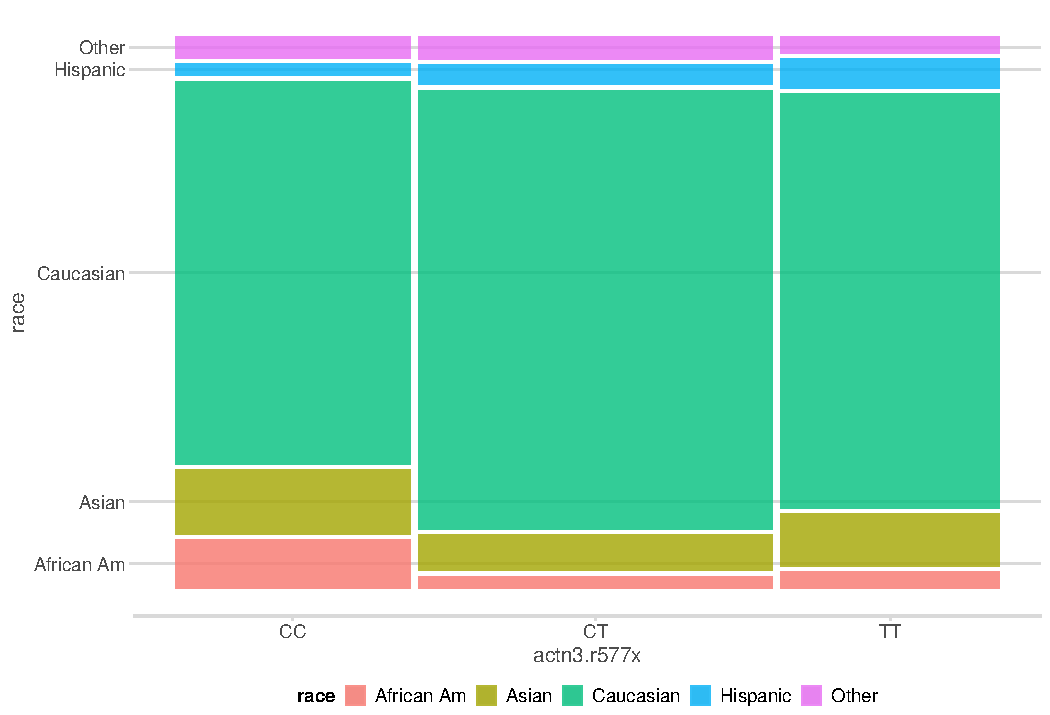
\includegraphics[width=\maxwidth]{figure/mosaic-1-1} 

}



\end{knitrout}
	
\end{frame}



\begin{frame}[fragile]{Mosaic plots - race, genotype and sex}
\begin{knitrout}\tiny
\definecolor{shadecolor}{rgb}{0.969, 0.969, 0.969}\color{fgcolor}\begin{kframe}
\begin{alltt}
    \hlkwd{ggplot}\hlstd{(}\hlkwc{data} \hlstd{= famuss)} \hlopt{+}
      \hlkwd{geom_mosaic}\hlstd{(}\hlkwd{aes}\hlstd{(}\hlkwc{x} \hlstd{=} \hlkwd{product}\hlstd{(race, actn3.r577x),}
                      \hlkwc{fill} \hlstd{= race,} \hlkwc{conds} \hlstd{=} \hlkwd{product}\hlstd{(sex)),}
                      \hlkwc{divider} \hlstd{=} \hlkwd{mosaic}\hlstd{(}\hlstr{"v"}\hlstd{))}
\end{alltt}
\end{kframe}

{\centering 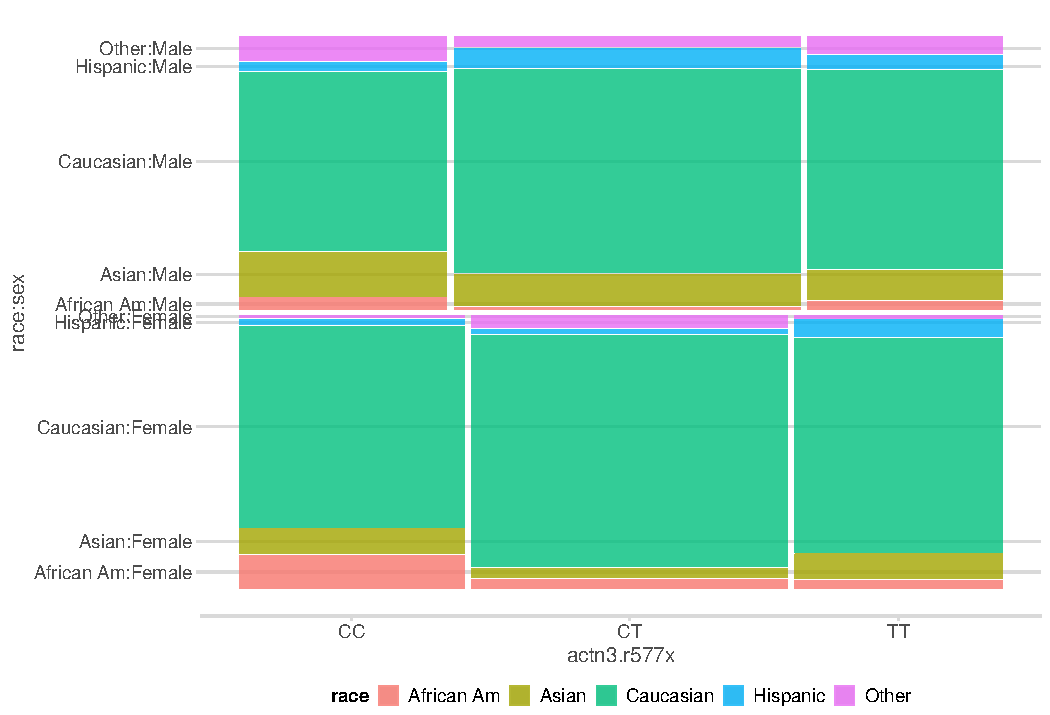
\includegraphics[width=\maxwidth]{figure/mosaic-2-1} 

}



\end{knitrout}
	
\end{frame}



\section{A numerical variable and a categorical variable}

\begin{frame}{A numerical variable and a categorical variable}
	\protect\hypertarget{a-numerical-variable-and-a-categorical-variable}{}
	
	\begin{itemize}
		\item \emph{FAMuSS} was designed to study the relationship between genotype at
	the location \emph{r577x} in the gene \emph{ACTN3} and muscle strength.
	
	\item Muscle strength was assessed by the percent change in non-dominant arm
	strength after resistance training (\texttt{ndrm.ch}).
	
	\item What visualization would be a good choice to make this comparison?
	\end{itemize}
	
\end{frame}


\begin{frame}[fragile]{A numerical variable and a categorical variable}
	\protect\hypertarget{a-numerical-variable-and-a-categorical-variable-1}{}
	
	\scriptsize
	
	\scriptsize
	

	
\begin{knitrout}\scriptsize
\definecolor{shadecolor}{rgb}{0.969, 0.969, 0.969}\color{fgcolor}\begin{kframe}
\begin{alltt}
\hlkwd{ggplot}\hlstd{(}\hlkwc{data} \hlstd{= famuss,} \hlkwc{mapping} \hlstd{=} \hlkwd{aes}\hlstd{(}\hlkwc{x} \hlstd{= actn3.r577x,} \hlkwc{y} \hlstd{= ndrm.ch,} \hlkwc{fill} \hlstd{= actn3.r577x))} \hlopt{+}
  \hlkwd{geom_boxplot}\hlstd{()}
\end{alltt}
\end{kframe}

{\centering 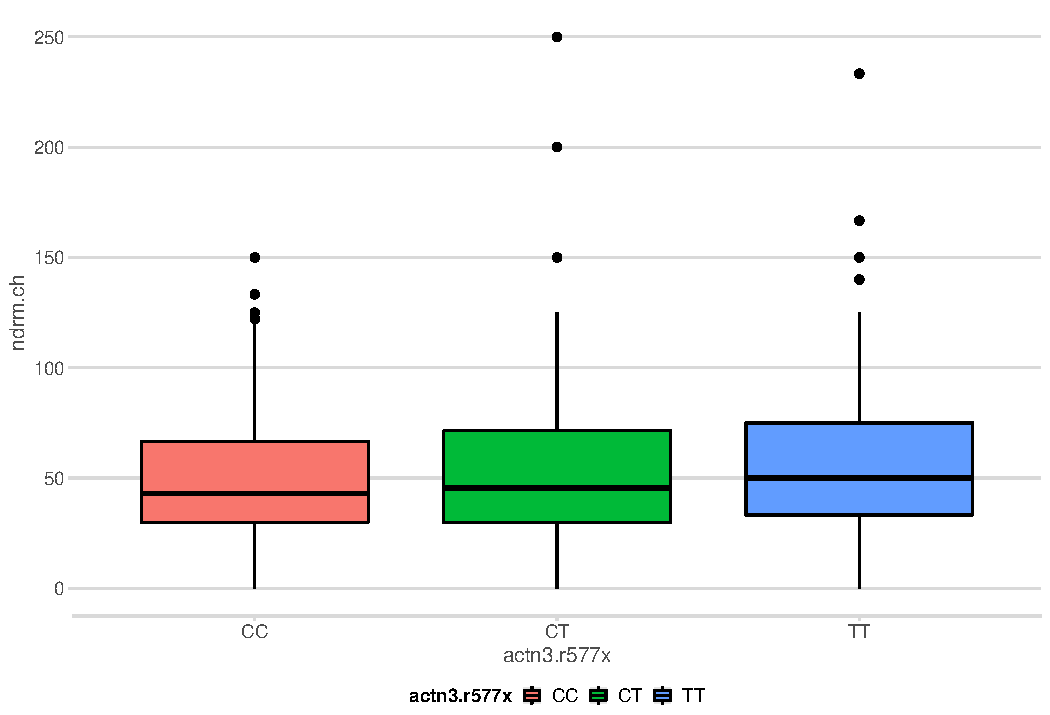
\includegraphics[width=\maxwidth]{figure/box-1-1} 

}



\end{knitrout}
	
	
	\normalsize
	
\end{frame}


\begin{frame}[fragile]{Correlations}
\begin{knitrout}\scriptsize
\definecolor{shadecolor}{rgb}{0.969, 0.969, 0.969}\color{fgcolor}\begin{kframe}
\begin{alltt}
\hlkwd{cor}\hlstd{(famuss}\hlopt{$}\hlstd{actn3.r577x, famuss}\hlopt{$}\hlstd{ndrm.ch)}
\end{alltt}


{\ttfamily\noindent\bfseries\color{errorcolor}{\#\# Error in cor(famuss\$actn3.r577x, famuss\$ndrm.ch): 'x' must be numeric}}\begin{alltt}
\hlkwd{cor}\hlstd{(}\hlkwd{as.numeric}\hlstd{(famuss}\hlopt{$}\hlstd{actn3.r577x), famuss}\hlopt{$}\hlstd{ndrm.ch,} \hlkwc{method} \hlstd{=} \hlstr{"pearson"}\hlstd{)}
\end{alltt}
\begin{verbatim}
## [1] 0.1
\end{verbatim}
\begin{alltt}
\hlkwd{cor}\hlstd{(}\hlkwd{as.numeric}\hlstd{(famuss}\hlopt{$}\hlstd{actn3.r577x), famuss}\hlopt{$}\hlstd{ndrm.ch,} \hlkwc{method} \hlstd{=} \hlstr{"kendall"}\hlstd{)}
\end{alltt}
\begin{verbatim}
## [1] 0.077
\end{verbatim}
\begin{alltt}
\hlkwd{cor}\hlstd{(}\hlkwd{as.numeric}\hlstd{(famuss}\hlopt{$}\hlstd{actn3.r577x), famuss}\hlopt{$}\hlstd{ndrm.ch,} \hlkwc{method} \hlstd{=} \hlstr{"spearman"}\hlstd{)}
\end{alltt}
\begin{verbatim}
## [1] 0.098
\end{verbatim}
\end{kframe}
\end{knitrout}
\end{frame}

\section{Summary}

\begin{frame}{Summary of exploring data slides} 
	
\begin{itemize}
	\item Two types of variables:
	\begin{itemize}
		\item \textbf{Numeric}: Discrete, Continuous
		\item \textbf{Categorical}: Ordinal, Nominal
	\end{itemize}
\pause
\item The collection of values for a numerical or categorical is called the distribution of that variable
\pause
\item Measures of center include mean and median. 
\item Measures of spread include standard deviation, interquartile range
\item Median and IQR are robust to outliers
\pause
\item Histograms, boxplots, violin plots, and scatterplots are useful graphical summaries of numerical data, which can also be grouped by a categorical variable
\item Bar plots, contingency tables, mosaic plots are useful summaries of categorical data
\end{itemize}
\end{frame}

\begin{frame}{Summary of exploring data slides \textit{continued}} 
	
	\begin{itemize}
		\item Correlation coefficient ($r$) quantifies the strength of a linear trend. 
		\item The \texttt{multiple R-squared} in a simple linear regression output is equal to $r^2$. 
		\item Transformation (e.g. log) can produce better linear associations for highly skewed data. But be careful about the interpretation!
		\pause
		\item Given a contingency table, the frequency distribution of one of the variables is called its marginal distribution
		\item Conditional distributions show the distribution of one variable for just those cases that satisfy a condition on another variable
		\item See \url{https://www.r-graph-gallery.com/} and \url{https://www.data-to-viz.com/} for a collection of graphical displays
	\end{itemize}
\end{frame}

\begin{frame}[fragile]{Session Info}
	\tiny
	
\begin{knitrout}\tiny
\definecolor{shadecolor}{rgb}{0.969, 0.969, 0.969}\color{fgcolor}\begin{kframe}
\begin{verbatim}
R version 4.0.2 (2020-06-22)
Platform: x86_64-pc-linux-gnu (64-bit)
Running under: Pop!_OS 20.10

Matrix products: default
BLAS:   /usr/lib/x86_64-linux-gnu/openblas-pthread/libblas.so.3
LAPACK: /usr/lib/x86_64-linux-gnu/openblas-pthread/libopenblasp-r0.3.10.so

attached base packages:
[1] tools     stats     graphics  grDevices utils     datasets  methods  
[8] base     

other attached packages:
 [1] ggmosaic_0.3.3      cowplot_1.1.0       openintro_2.0.0    
 [4] usdata_0.1.0        cherryblossom_0.1.0 airports_0.1.0     
 [7] oibiostat_0.2.0     NCStats_0.4.7       FSA_0.8.30         
[10] forcats_0.5.0       stringr_1.4.0       dplyr_1.0.2        
[13] purrr_0.3.4         readr_1.4.0         tidyr_1.1.2        
[16] tibble_3.0.6        ggplot2_3.3.3       tidyverse_1.3.0    
[19] knitr_1.31         

loaded via a namespace (and not attached):
  [1] minqa_1.2.4        TH.data_1.0-10     colorspace_2.0-0  
  [4] ellipsis_0.3.1     rio_0.5.16         leaflet_2.0.3     
  [7] sjlabelled_1.1.7   snakecase_0.11.0   estimability_1.3  
 [10] ggstance_0.3.4     parameters_0.8.6   ggdendro_0.1.22   
 [13] fs_1.5.0           rstudioapi_0.13    farver_2.0.3      
 [16] ggrepel_0.8.2      mvtnorm_1.1-1      lubridate_1.7.9   
 [19] xml2_1.3.2         codetools_0.2-16   mosaic_1.7.0      
 [22] splines_4.0.2      sjmisc_2.8.5       polyclip_1.10-0   
 [25] jsonlite_1.7.2     nloptr_1.2.2.2     ggeffects_0.16.0  
 [28] broom_0.7.2        dbplyr_1.4.4       ggforce_0.3.2     
 [31] effectsize_0.3.3   compiler_4.0.2     httr_1.4.2        
 [34] productplots_0.1.1 sjstats_0.18.0     emmeans_1.5.1     
 [37] backports_1.2.1    lazyeval_0.2.2     assertthat_0.2.1  
 [40] Matrix_1.2-18      cli_2.3.0          tweenr_1.0.1      
 [43] htmltools_0.5.1.1  coda_0.19-4        gtable_0.3.0      
 [46] glue_1.4.2         Rcpp_1.0.6         carData_3.0-4     
 [49] cellranger_1.1.0   vctrs_0.3.6        sjPlot_2.8.5      
 [52] nlme_3.1-149       crosstalk_1.1.0.1  insight_0.9.6     
 [55] xfun_0.21          ps_1.5.0           lme4_1.1-23       
 [58] openxlsx_4.1.5     rvest_0.3.6        lifecycle_1.0.0   
 [61] mosaicCore_0.8.0   pacman_0.5.1       statmod_1.4.34    
 [64] zoo_1.8-8          MASS_7.3-53        scales_1.1.1      
 [67] hms_0.5.3          sandwich_2.5-1     RColorBrewer_1.1-2
 [70] curl_4.3           mosaicData_0.20.1  gridExtra_2.3     
 [73] TeachingDemos_2.12 stringi_1.5.3      highr_0.8         
 [76] bayestestR_0.7.2   boot_1.3-25        zip_2.1.1         
 [79] rlang_0.4.10       pkgconfig_2.0.3    evaluate_0.14     
 [82] lattice_0.20-41    htmlwidgets_1.5.3  labeling_0.4.2    
 [85] tidyselect_1.1.0   ggformula_0.9.4    plyr_1.8.6        
 [88] magrittr_2.0.1     R6_2.5.0           generics_0.1.0    
 [91] multcomp_1.4-13    DBI_1.1.0          pillar_1.4.7      
 [94] haven_2.3.1        foreign_0.8-80     withr_2.4.1       
 [97] survival_3.2-3     abind_1.4-5        performance_0.5.0 
[100] modelr_0.1.8       crayon_1.4.1       car_3.0-9         
[103] plotly_4.9.2.1     grid_4.0.2         readxl_1.3.1      
[106] data.table_1.13.6  blob_1.2.1         reprex_0.3.0      
[109] digest_0.6.27      xtable_1.8-4       munsell_0.5.0     
[112] viridisLite_0.3.0 
\end{verbatim}
\end{kframe}
\end{knitrout}
	
\end{frame}

\end{document}	
	
\hypertarget{case-study-molecular-cancer-classification}{%
\section{Case study: molecular cancer classification}\label{case-study-molecular-cancer-classification}}
						
\begin{frame}{The potential value of genomic data in cancer}
							\protect\hypertarget{the-potential-value-of-genomic-data-in-cancer}{}
							
							The majority of cancers are diagnosed by an expert pathologist examining
							slides of malignant cells.
							
							Can that be done more accurately by characterizing the genetic makeup of
							the malignancy?
							
							\begin{itemize}
								\tightlist
								\item
								This is perhaps the major potential of genomic characterizations of
								tumors.
							\end{itemize}
							
							There are many forms of childhood leukemia.
							
							\begin{itemize}
								\item
								Acute myeloblastic leukemia (AML) and acute lymphoblastic leukemia
								(ALL) are the most common.
								\item
								AML is a cancer of the bone marrow, where white blood cells
								(lymphocytes) are produced.
								\item
								ALL is a cancer of the lymphocytes and is designated as B-cell (ALLB)
								or T-cell (ALLT).
							\end{itemize}
							
\end{frame}


		
\begin{frame}{Prognosis of the two cancers}
							\protect\hypertarget{prognosis-of-the-two-cancers}{}
							
							The probability that a child diagnosed with ALL is survives at least 5
							years after the diagnosis is approximately 90\%.
							
							Approximately 65\% of children diagnosed with AML survive at least 5
							years.
							
							The diagnosis of leukemia type determines the therapy that will be given
							to the child, and the successful treatments for ALL and AML are
							different.
							
							In 1999, Todd Golub from the Dana-Farber and the Broad Institute
							examined the possibility of classifying leukemia through using a genetic
							analysis of a blood sample.
							
						\end{frame}
						
						\begin{frame}{Analyzing the Golub data}
							\protect\hypertarget{analyzing-the-golub-data}{}
							
							We can re-analyze the Golub data using tools from graphical and
							numerical summaries.
							
							Our analysis will not be identical to the Golub analysis, but will be
							similar in spirit.
							
							The tools are straighforward\ldots   
							
							\begin{itemize}
								\item
								Thinking through the problem and assembling the tools is the hard
								part.
								\item
								The process is more important than the final recipe.
							\end{itemize}
							
						\end{frame}
						
						\begin{frame}{Gene expression (details in \emph{OI Biostat})}
							\protect\hypertarget{gene-expression-details-in-oi-biostat}{}
							
							\small
							
							\begin{itemize}
								\item
								The genetic code stored in DNA contains the information for producing
								the proteins that determine an organism's phenotype.
								\item
								Genes that are transcriptionally active (i.e.~turned ``on'') are
								transcribed into messenger RNA (mRNA) that gets translated into
								proteins.
								\item
								Genes can be switched on or off, and expressed at varying levels.
								Variations in gene expression produce the range of physical,
								biochemical, and developmental differences in cells and tissues.
								\item
								Quantifying the amount of RNA produced in a cell allows for a measure
								of gene expression.
								\item
								The transcriptome, or expression profile, is the complete set of RNA
								transcripts produced by the genome in a cell or set of cells.
							\end{itemize}
							
						\end{frame}
						
						\begin{frame}{Microarrays (details in \emph{OI Biostat})}
							\protect\hypertarget{microarrays-details-in-oi-biostat}{}
							
							\small
							
							\begin{itemize}
								\item
								Microarray technology is based on hybridization between two DNA
								strands, in which complementary nucleotide sequences specifically pair
								together.
								\item
								The mRNA from a sample is converted into complementary-DNA (cDNA),
								labeled with a fluorescent dye, and added to the microarray.
								\item
								When cDNA from the sample encounters complementary DNA probes, the two
								strands will hybridize, allowing the cDNA to adhere to specific spots
								on the slide.
								\item
								When the chip is illuminated and scanned, the intensity of
								fluorescence detected at each spot corresponds to the amount of bound
								cDNA.
								\item
								DNA microarrays do not directly quantify gene expression levels or
								quantity of mRNA present in a sample.
								\item
								The fluorescence intensity data only provide a relative measure of
								gene expression, showing which genes on the chip seem to be more or
								less active in relation to each other.
							\end{itemize}
							
						\end{frame}
						
						\begin{frame}{Microarrays}
							\protect\hypertarget{microarrays}{}
							
							\begin{figure}
								\centering
								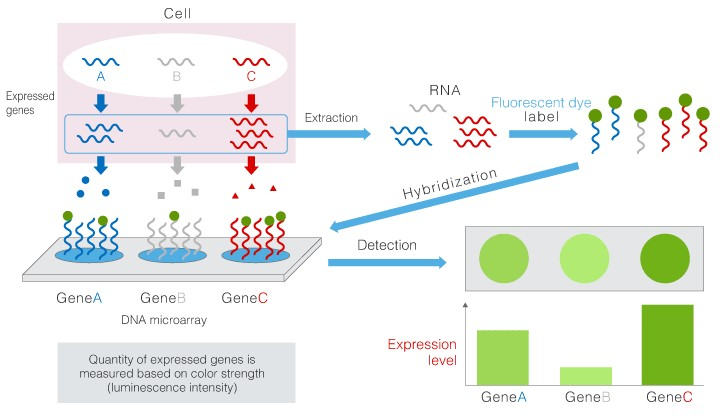
\includegraphics[scale=0.5]{figures/microarray_schematic.jpg}
								\caption{fluorescence detection}
							\end{figure}
							
						\end{frame}
						
						\begin{frame}{The Golub clinical data}
							\protect\hypertarget{the-golub-clinical-data}{}
							
							Demographic variables described in \emph{OI Biostat} Table 1.54:
							
							\scriptsize
							
							\begin{longtable}[]{@{}ll@{}}
								\toprule
								\begin{minipage}[b]{0.12\columnwidth}\raggedright
									Variable\strut
								\end{minipage} & \begin{minipage}[b]{0.82\columnwidth}\raggedright
									Description\strut
								\end{minipage}\tabularnewline
								\midrule
								\endhead
								\begin{minipage}[t]{0.12\columnwidth}\raggedright
									Samples\strut
								\end{minipage} & \begin{minipage}[t]{0.82\columnwidth}\raggedright
									Sample or chip number. The material from each patient was examined on a
									separate chip and experimental run.\strut
								\end{minipage}\tabularnewline
								\begin{minipage}[t]{0.12\columnwidth}\raggedright
									BM.PB\strut
								\end{minipage} & \begin{minipage}[t]{0.82\columnwidth}\raggedright
									Type of patient material. BM denotes bone marrow; PB denotes a
									peripheral blood sample.\strut
								\end{minipage}\tabularnewline
								\begin{minipage}[t]{0.12\columnwidth}\raggedright
									Gender\strut
								\end{minipage} & \begin{minipage}[t]{0.82\columnwidth}\raggedright
									F for female, M for male.\strut
								\end{minipage}\tabularnewline
								\begin{minipage}[t]{0.12\columnwidth}\raggedright
									Source\strut
								\end{minipage} & \begin{minipage}[t]{0.82\columnwidth}\raggedright
									Hospital where the patient was treated.\strut
								\end{minipage}\tabularnewline
								\begin{minipage}[t]{0.12\columnwidth}\raggedright
									tissue.mf\strut
								\end{minipage} & \begin{minipage}[t]{0.82\columnwidth}\raggedright
									A variable showing the combination of type of patient material and sex
									of the patient. BM:f denotes bone marrow from a female patient,
									etc.\strut
								\end{minipage}\tabularnewline
								\begin{minipage}[t]{0.12\columnwidth}\raggedright
									cancer\strut
								\end{minipage} & \begin{minipage}[t]{0.82\columnwidth}\raggedright
									The type of leukemia; aml is acute myeloblastic leukemia, allB is acute
									lymphoblastic leukemia which started in B-cells (cells that mature into
									plasma cells) origin, and allT is acute lymphoblastic leukemia with
									T-cell origin (T-cells are a type of white blood cell).\strut
								\end{minipage}\tabularnewline
								\bottomrule
							\end{longtable}
							
						\end{frame}
						
						\begin{frame}{The Golub expression data}
							\protect\hypertarget{the-golub-expression-data}{}
							
							The expression data is contained in the last 7,129 columns.
							
							Each column is a variable with a name corresponding to the name of the
							probe on the microarray.
							
							The expression levels record fluorescence intensity for each gene.
							
							\begin{itemize}
								\item
								The intensity levels have no inherent biological meaning.
								\item
								Data have been normalized to adjust for variability between the
								separate arrays used for each patient.
							\end{itemize}
							
						\end{frame}
						
						\begin{frame}{Selected variables and columns from Golub data}
							\protect\hypertarget{selected-variables-and-columns-from-golub-data}{}
							
							\captionsetup[table]{labelformat=empty}
							\scriptsize
							
							\scriptsize
							
							\begin{longtable}[]{@{}rllrrr@{}}
								\caption{\emph{OI Biostat} Table 1.40}\tabularnewline
								\toprule
								Samples & Gender & cancer & AFFX-BioB-5\_at & AFFX-BioB-M\_at &
								AFFX-BioB-3\_at\tabularnewline
								\midrule
								\endfirsthead
								\toprule
								Samples & Gender & cancer & AFFX-BioB-5\_at & AFFX-BioB-M\_at &
								AFFX-BioB-3\_at\tabularnewline
								\midrule
								\endhead
								39 & F & allB & -1363.28 & -1058.59 & -541.47\tabularnewline
								40 & F & allB & -796.29 & -1167.10 & 7.54\tabularnewline
								42 & F & allB & -679.14 & -1069.83 & -690.30\tabularnewline
								47 & M & allB & -1164.40 & -1109.94 & -990.13\tabularnewline
								48 & F & allB & -1299.65 & -1402.00 & -1077.54\tabularnewline
								\bottomrule
							\end{longtable}
							
							\normalsize
							
						\end{frame}
						
						\begin{frame}{Analyzing the Golub leukemia data}
							\protect\hypertarget{analyzing-the-golub-leukemia-data}{}
							
							We will do an analysis in class using some of the simple but
							surprisingly powerful ideas behind numerical and graphical summaries.
							
							The goal of the Golub study was to develop a procedure for
							distinguishing between AML and ALL based only on the gene expression
							levels of a patient. There are two major issues to be addressed:
							
							\begin{enumerate}
								\item
								Which genes are the most informative for making a prediction?
								\item
								What is a workable strategy for predicting leukemia type from
								expression data for a specific set of genes?
							\end{enumerate}
							
						\end{frame}
						
						\begin{frame}[fragile]{Starting small\ldots{}}
							\protect\hypertarget{starting-small}{}
							
							\footnotesize
							
							\scriptsize
							
\begin{verbatim}
##    cancer        A         B        C        D
## 69   allB 39307.96 35232.401 41170.76 35792.79
## 67   allT 32281.88 41432.024 59328.51 49608.14
## 55   allB 47429.94 35568.928 56074.96 42857.78
## 56   allB 25533.87 16983.749 28056.75 32693.92
## 59   allB 35960.55 24191.746 27637.90 22240.75
## 52    aml 46177.95  6189.465 12557.24 34485.41
## 53    aml 43790.70 33661.825 38380.30 29758.25
## 51    aml 53420.05 26109.245 31427.20 23809.70
## 50    aml 41241.59 37589.773 47325.77 30099.36
## 54    aml 41300.57 49198.412 66026.10 56248.62
\end{verbatim}
\end{frame}
						



%\begin{frame}[allowframebreaks]
%\nocite{breiman1984classification}
%	\nocite{friedman2001elements}
%	\nocite{james2013introduction}
%	\nocite{lopez2015arbres}
%	\frametitle{References}
%\printbibliography
%\end{frame}




\end{document}
